\documentclass{beamer}
\RequirePackage{luatex85}

% Style
\usepackage{xcolor}

\usetheme{Madrid}
\usepackage{dirtree}
% Color
\definecolor{flatblue}{RGB}{106, 137, 204}
\usecolortheme[named=flatblue]{structure}
% Font
\usepackage{emoji}
\usepackage{fontspec}
\usepackage{csquotes}
\setsansfont{Garamond Libre}
% Code
\usepackage{listings}
\usepackage{graphicx}
\usepackage{hyperref}
\hypersetup{
    colorlinks=true,
    linkcolor=flatblue,
    filecolor=flatblue,
    urlcolor=flatblue,
    citecolor=flatblue
}
\definecolor{flatgreen}{RGB}{0, 98, 102}
\definecolor{flatgreyish}{RGB}{209, 216, 224}
\lstset{
    basicstyle=\ttfamily\scriptsize,
    backgroundcolor=\color{flatgreyish},
    keywordstyle=\color{flatgreen},        % Keywords font ('*' = uppercase)
    commentstyle=\color{flatblue},         % Step between two line-numbers
    columns=fullflexible,
    breaklines=true
}

% Highlight
\usepackage[most]{tcolorbox}
\usepackage{cleveref}
\crefformat{footnote}{#2\footnotemark[#1]#3}
\usepackage{amsmath}
\usepackage{wasysym}
\definecolor{flatorange}{RGB}{255, 165, 2}
\definecolor{flatred}{RGB}{255, 71, 87}
\tcbset{textmarker/.style={%
skin=enhancedmiddle jigsaw,breakable,parbox=false,
boxrule=0mm,leftrule=2mm,rightrule=0mm,boxsep=0mm,arc=0mm,outer arc=0mm,
left=1mm,right=1mm,top=1mm,bottom=1mm,toptitle=1mm,bottomtitle=1mm}}
\newtcolorbox{dangercolorbox}{textmarker,colback=flatorange,colframe=flatred}

% Title
\title{Architectures d’Applications - Bachelor CSI}
\author{Christophe Brun}
\institute{Campus Saint-Michel IT}
\date{03 avril 2024}
\beamertemplatenavigationsymbolsempty

% Graphix with arrows in between
\newcommand*{\vcenterimage}[1]{\vcenter{\hbox{\includegraphics[width=5cm]{#1}}}}
\newcommand*{\vcenterarrow}{\vcenter{\hbox{$\Longrightarrow$}}}

\titlegraphic{
    \bigbreak
    
\includegraphics[width=2cm]{image/logo-papit}
    
\includegraphics[width=2cm]{image/logo-campus-saint-michel-it}
}
\begin{document}

    \begin{frame}
        \transdissolve
        \titlepage
    \end{frame}

    \begin{frame}{Table des matières}
        \tableofcontents
    \end{frame}


    \section{Programme du module}\label{sec:programme-du-module}
    \begin{frame}
        \frametitle{Architectures d’Applications}
        \framesubtitle{Compétence acquise aucours des 3 jours du module}
        \transdissolve
        Compétence~:
        \begin{itemize}
            \item \textquote{Concevoir une architecture d’applications.}~???
        \end{itemize}
        \pause
        \bigbreak
        Reformulation possible~:
        \begin{itemize}
            \item Concevoir une application architecturée.
        \end{itemize}
        \centering
        
\includegraphics[width=5cm]{image/engraving-of-a-monk-drawing-a-cathedral}
    \end{frame}

    \begin{frame}
        \frametitle{Architectures d’Applications}
        \framesubtitle{Le programme officiel des 3 jours du module}
        \transdissolve
        \fontsize{8pt}{8pt}\selectfont
        \begin{enumerate}
            \item Les différentes architectures d’une application
            \item L’architecture REST
            \begin{itemize}
                \fontsize{8pt}{8pt}\selectfont
                \item Architectures Orientées Services
                \begin{itemize}
                    \item Besoins de la SOA
                    \item Notion de service
                    \item Introduction aux Architectures Orientées Services
                \end{itemize}
                \item Vers les Architectures Orientées Services
                \begin{itemize}
                    \item Les architectures Client-Serveur
                    \item Les architectures Web
                \end{itemize}
                \item Les Web Services
                \begin{itemize}
                    \item Appel de procédure
                    \item World Wide Web
                    \item Formats d’échange textuels
                    \item Vers la notion de Web Service
                \end{itemize}
                \item Web Service de type SOAP et REST
                \item Guidelines API-REST
                \begin{itemize}
                    \item Gestion des actions et des URLs
                    \item Recherche, Tri, Filtre et Pagination
                    \item Gestion des erreurs
                \end{itemize}
            \end{itemize}
        \end{enumerate}
    \end{frame}

    \begin{frame}
        \transdissolve
        \frametitle{Evaluation}
        \begin{itemize}
            \item Bons points tout au long du module.
            \item 25 \% x 3 sur chaque séance de travaux dirigés évalués en fin de séance.
            Et une application orientée web REST ou SOAP~.
            \item 25 \% sur une évaluation écrite finale
        \end{itemize}
    \end{frame}

    \begin{frame}
        \transdissolve
        \frametitle{Intervenant sur le module architecture d'Aplication}
        \framesubtitle{Christophe Brun, conseil en développement informatique}

        \begin{columns}
            \column{0.7\textwidth}
            \begin{itemize}
                \item 1\textsuperscript{ere} année d'intervenant à Saint-Michel \emoji{star-struck}.

                \item 7 ans de conseil en développement au sein d'SSII~.

                \item 7 ans de conseil en développement à mon compte \href{https://papit.fr}{PapIT}.

                \item Passionné~!
                \bigbreak
                \begin{columns}
                    \column{0.5\textwidth}
                    \centering
                    
\includegraphics[width=3cm]{image/logo-uppa}
                    \column{0.5\textwidth}
                    \centering
                    
\includegraphics[width=3cm]{image/logo-universite-bordeaux}
                \end{columns}
            \end{itemize}
            \column{0.3\textwidth}
            \centering
            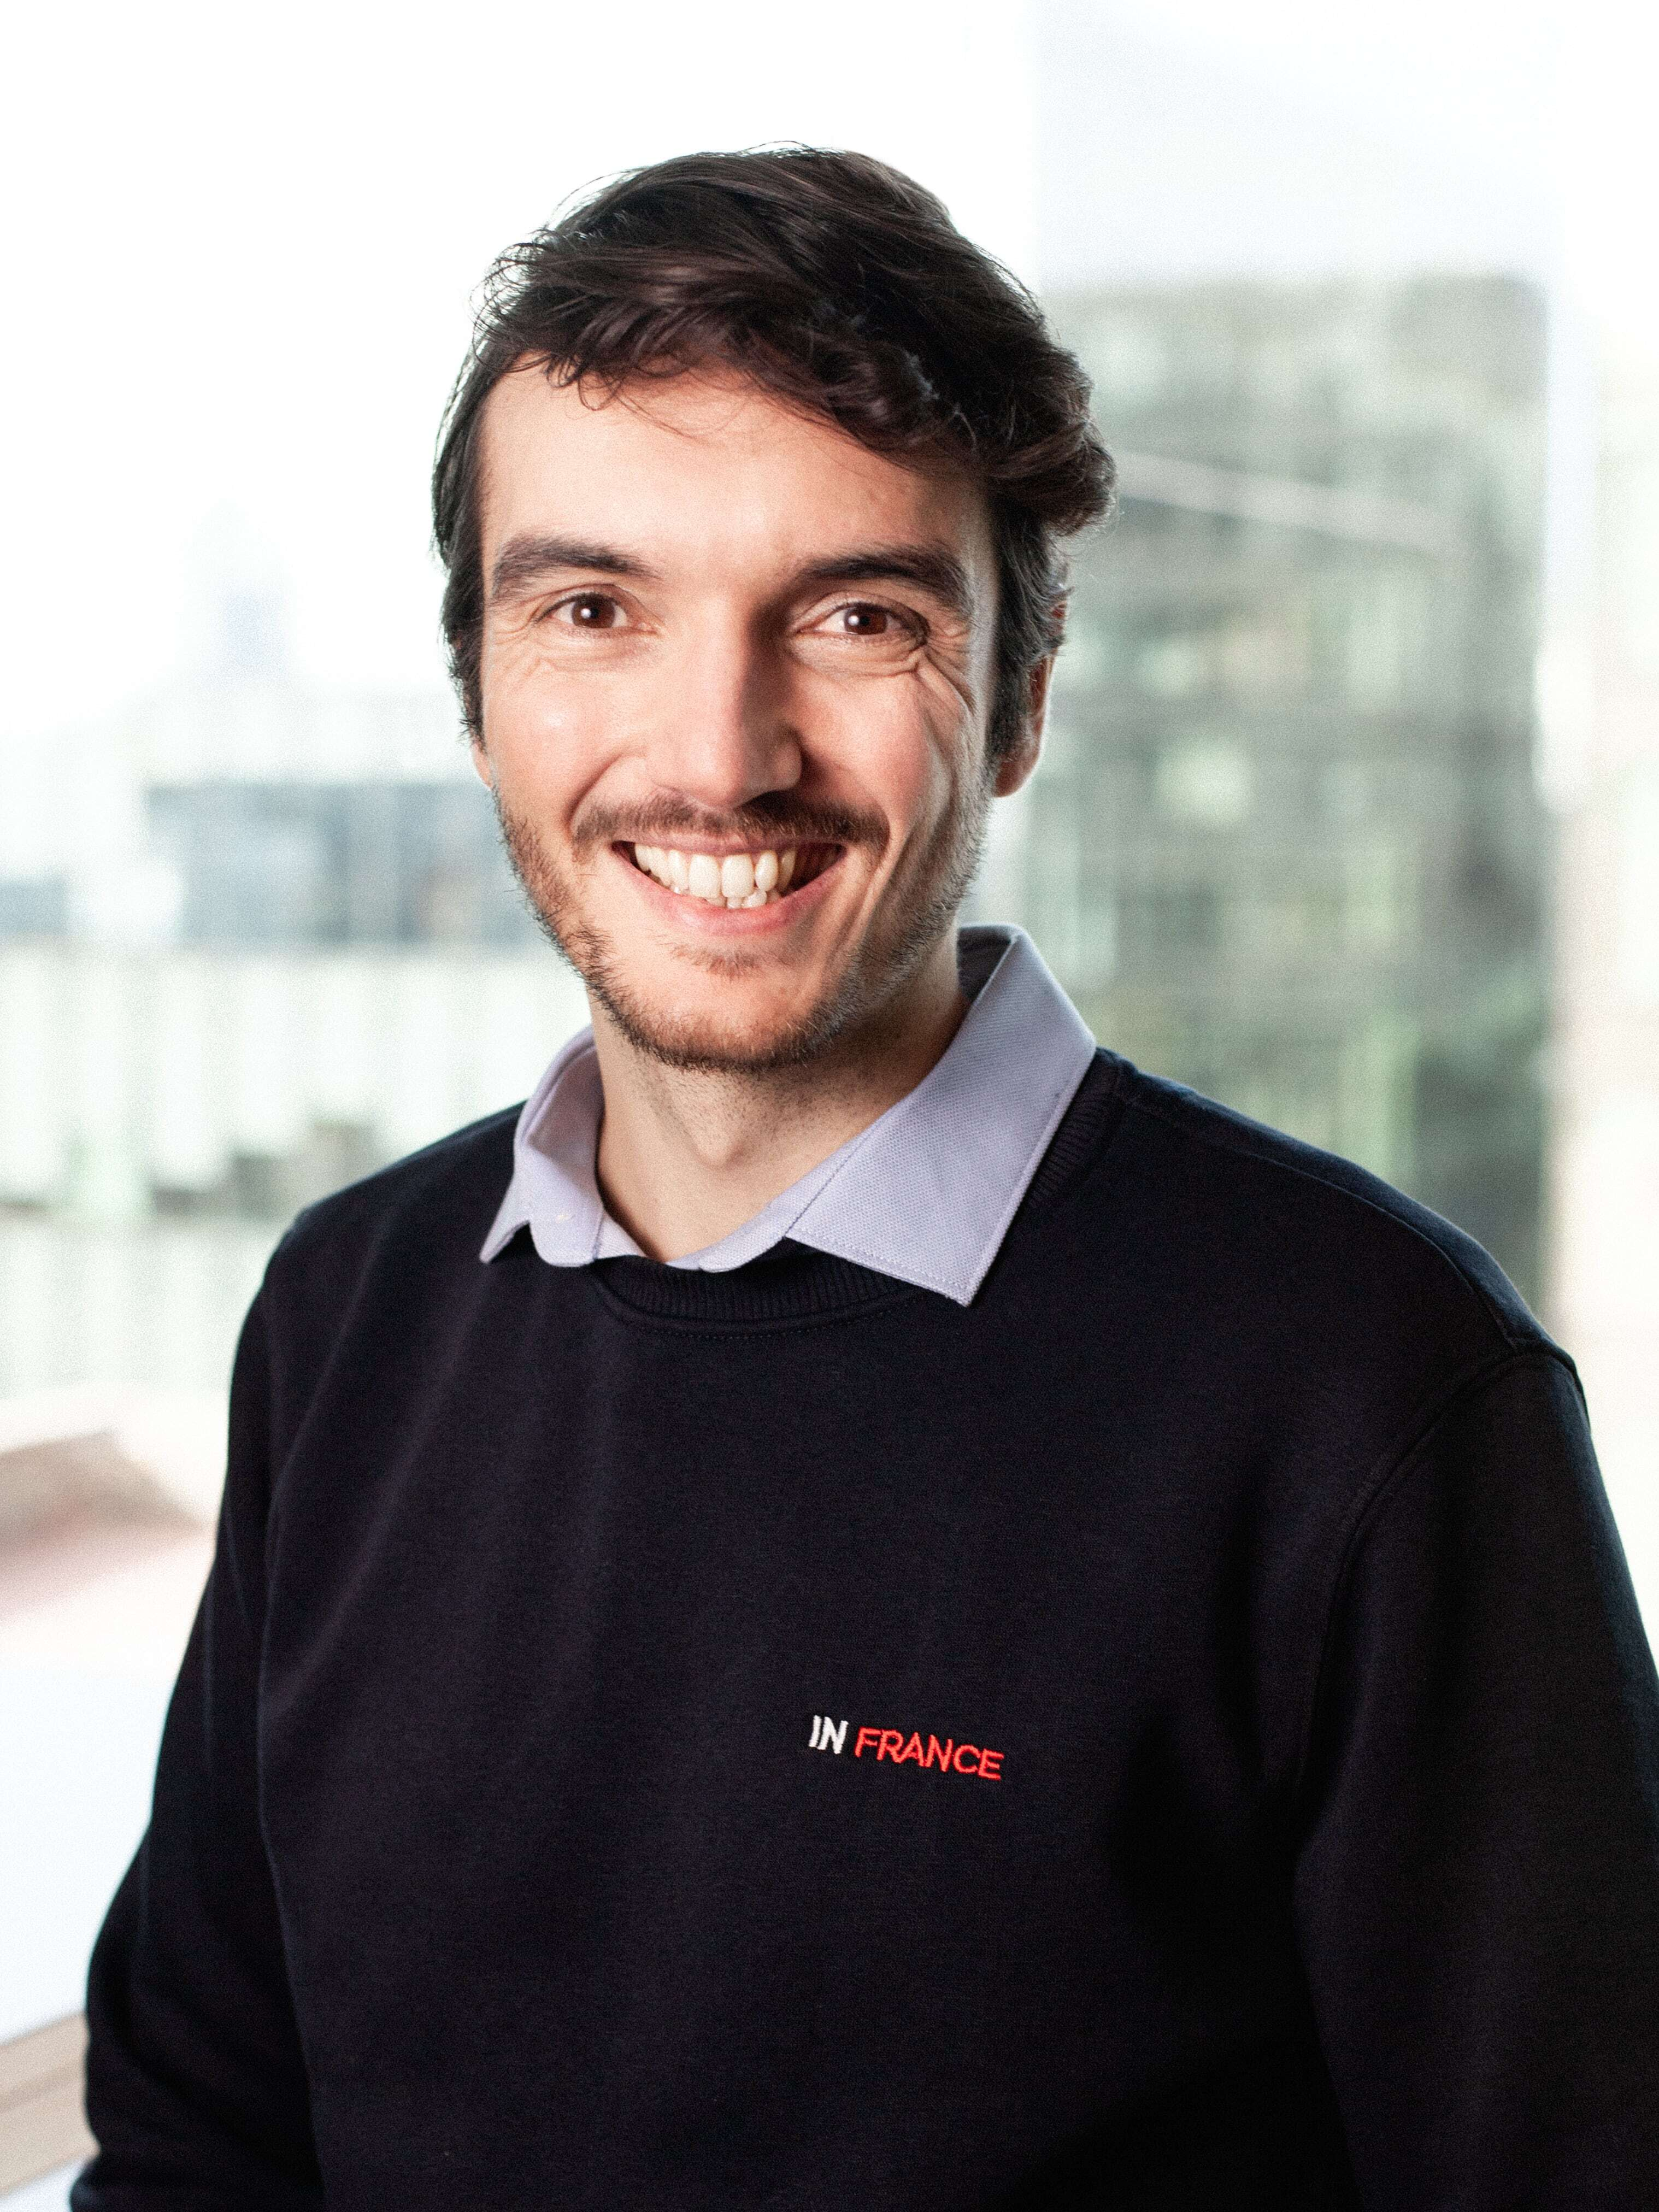
\includegraphics[width=5cm]{image/trombine-christophe}
        \end{columns}
    \end{frame}


    \section{Généralités}\label{sec:generalites}

    \begin{frame}
        \transdissolve
        \frametitle{Pourquoi le design ou architecture logicielle~?}
        \begin{columns}
            \column{0.5\textwidth}
            \textquote{The goal of software architecture is to minimize the human resources required to build and maintain the required system.}\footnotemark
            \centering
            \column{0.5\textwidth}
            \centering
            \begin{tabular}{cc}
                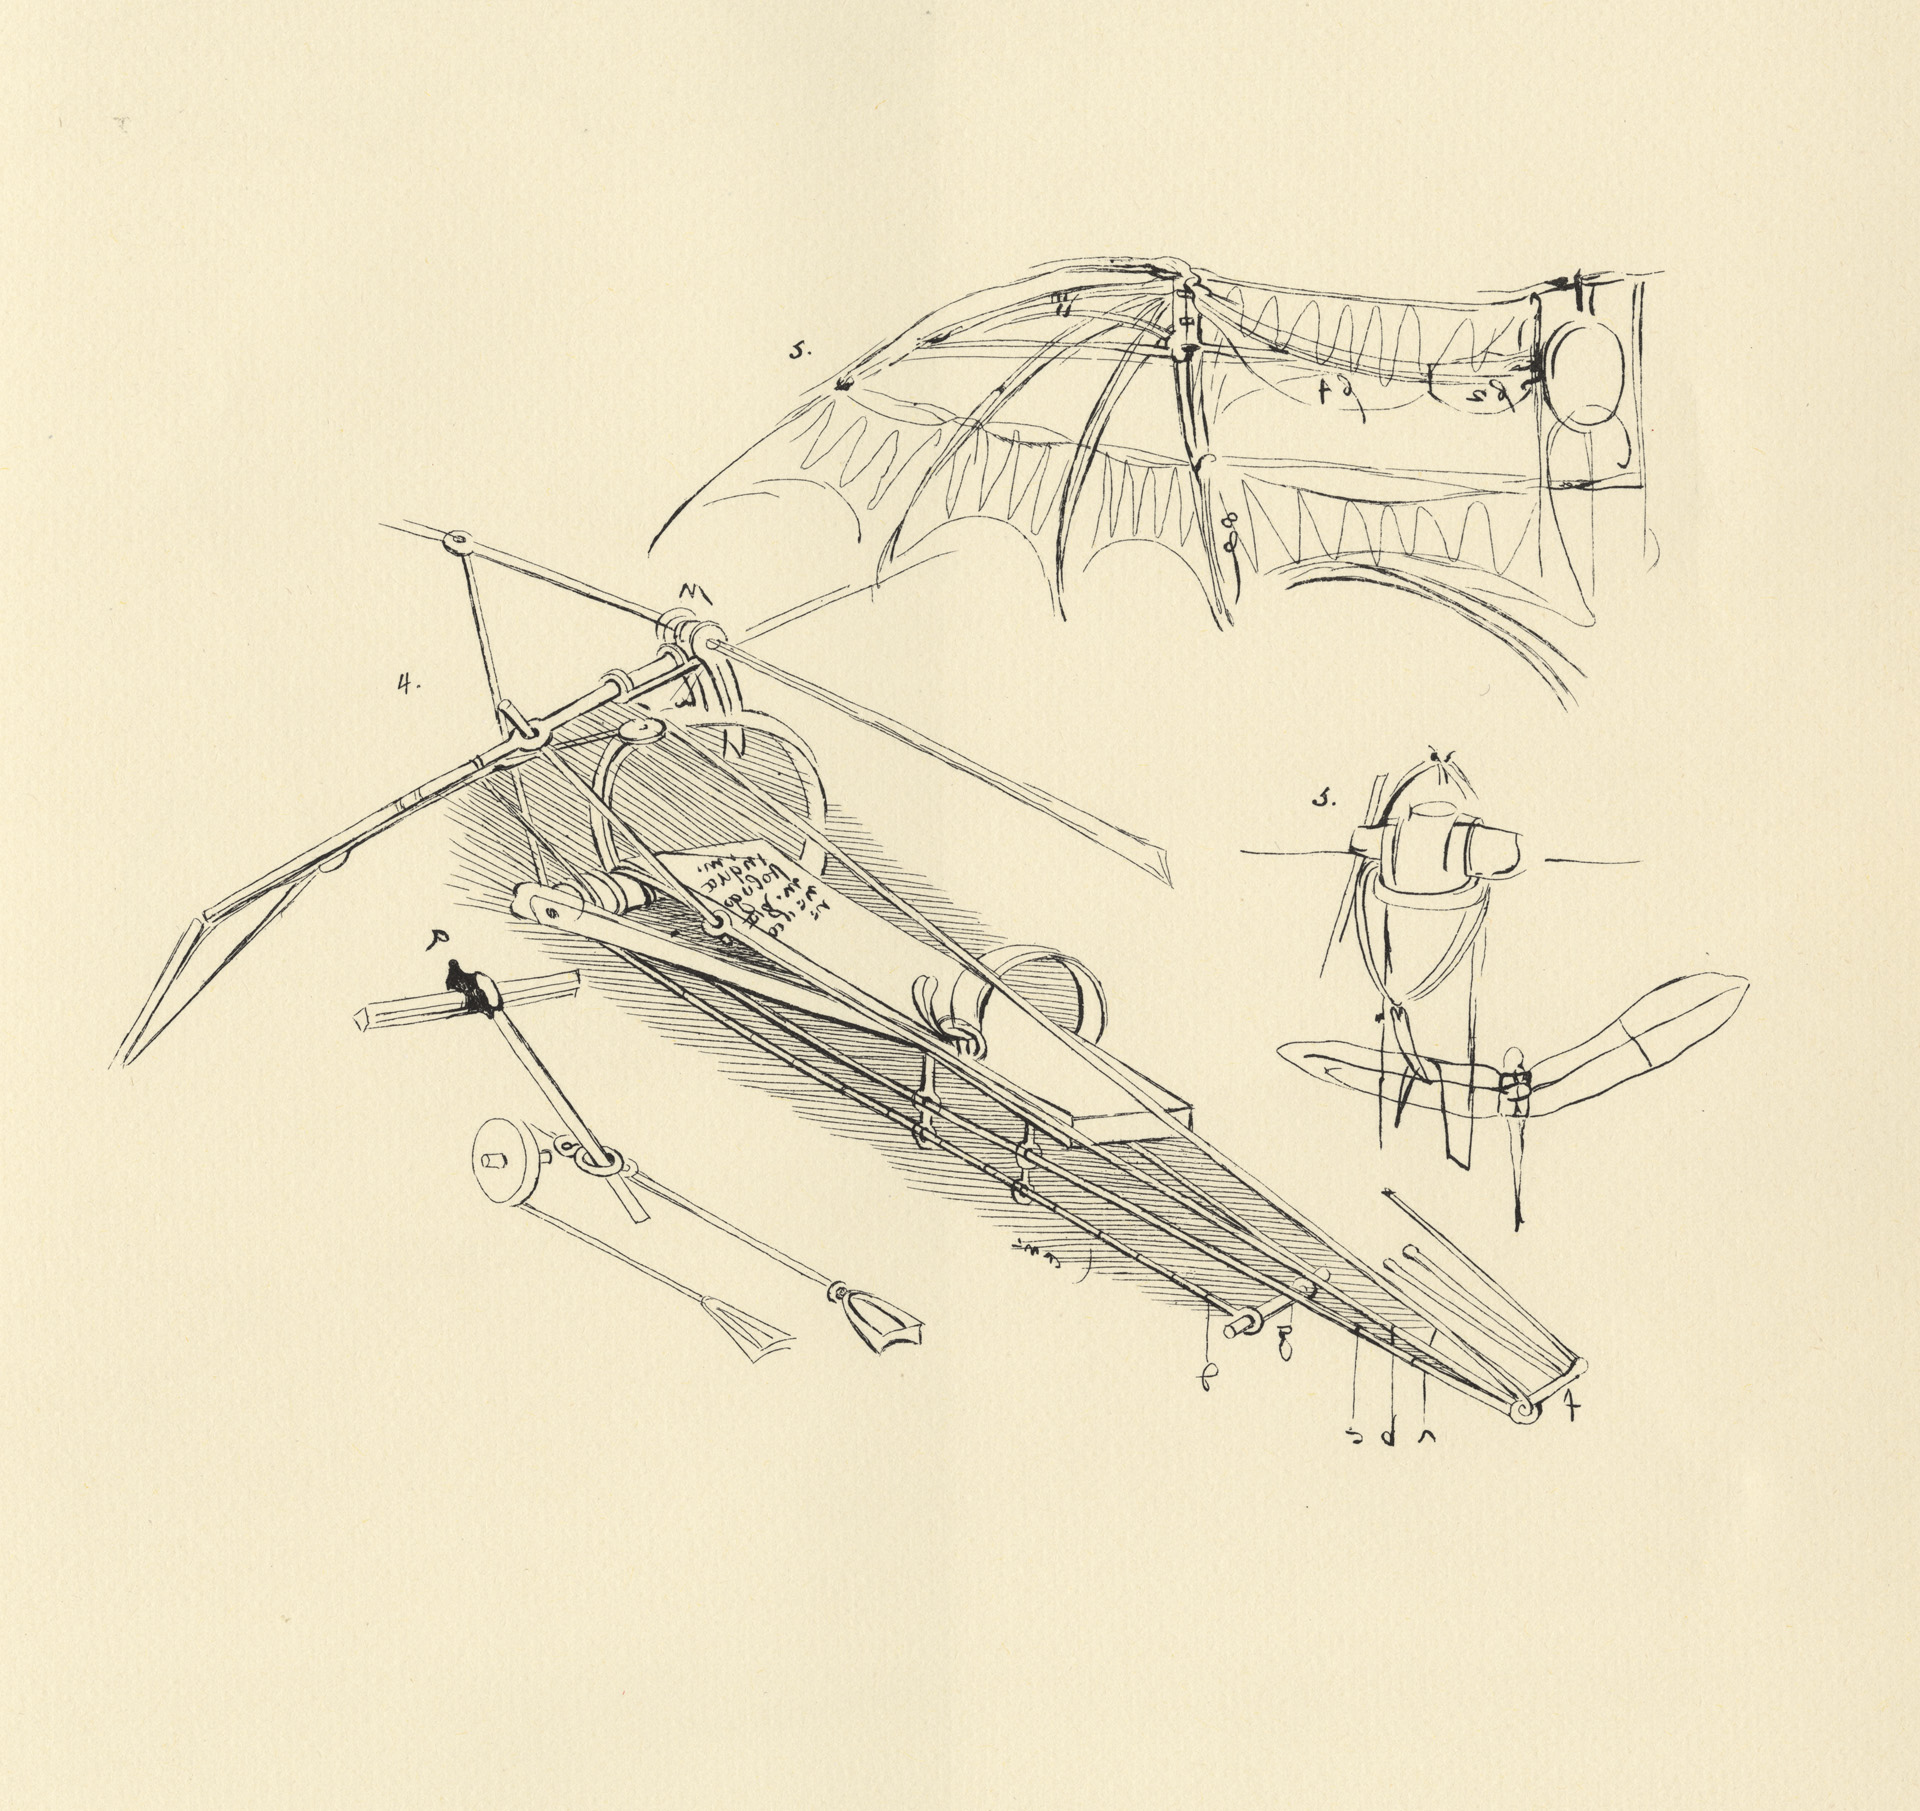
\includegraphics[width=6.0cm]{image/da-vinci-plans} \\
                L. de Vinci par C. G. Gerli en 1789.                \\
            \end{tabular}
        \end{columns}
        \footnotetext{\label{cleanarchitecture}Clean architecture, Robert C. Martin}
    \end{frame}

    \begin{frame}
        \transdissolve
        \frametitle{Éloge de la simplicité}
        Léonard de Vinci, 1452-1519~: \textquote{La simplicité est la sophistication suprême.}\footnote{La Pause Philo, \url{https://lapausephilo.fr/2015/09/15/simplicite-sophistication-supreme-leonard-de-vinci/}}
        \bigbreak
        Albert Einstein, 1879-1955~: \textquote{Si vous ne pouvez expliquer quelque chose simplement, c’est que vous ne l’avez pas bien compris.}
        \bigbreak
        Trouver et implémenter une architecture logicielle doit être simple.
        C'est compliqué il y a un souci.
        \bigbreak La modularité est en autre permise par la dissection d'un système complexe en sous-systèmes plus simples.
        Ces systèmes plus simples n'ont qu'une seule responsabilité (Comme en programmation fonctionnelle~?).
    \end{frame}

    \begin{frame}
        \transdissolve
        \frametitle{Définition}
        \framesubtitle{Architecture~?, Design~?, les deux~?}
        Encore une fois, pour faire simple, nous allons présumer que l'architecture et le design sont la même chose dans le monde du logiciel.\cref{cleanarchitecture}
        Le \textquote{Design patterns}\footnote{Design patterns, \url{https://refactoring.guru/design-patterns}} est un classique en développement logiciel.
        \bigbreak
        \textquote{The only way to go fast is to go well.}\cref{cleanarchitecture} Qu'est-ce que cela veut dire~?
        \bigbreak
        \textquote{The blueprint of the system.}\footnote{\label{fundsofsoftarch}Fundamentals of Software Architecture, Mark Richards et Neal Ford}
        \bigbreak
        Le mot système revient souvent.
        C'est un terme vague et récursif.
        C'est-à-dire qu'un système est composé de systèmes plus simples.
        L'architecture système est d'ailleurs un domaine en charge de l'architecture de l'entreprise, des produits et des logiciels.
    \end{frame}

    \begin{frame}
        \transdissolve
        \frametitle{Définition}
        \framesubtitle{Le couplage}
        C'est un des termes les plus importants en architecture logicielle.
        Il faut comprendre comment l'éviter tant que possible.
        \bigbreak
        \textquote{It is a result of putting a variable, constant, or function in a temporary convinient, thought inappropriate, location. This is lazy and careless}\footnote{\label{cleancode}Robert C. Martin, Clean Code}
    \end{frame}


    \section{Les briques}\label{sec:les-briques}

    \subsection{Généralités}\label{subsec:briques-generalites}
    \begin{frame}
        \transdissolve
        \frametitle{Les briques}
        \framesubtitle{Les briques en architecture}
        \begin{columns}
            \column{0.6\textwidth}
            Probablement hérité du jargon de l'architecture des bâtiments, le mot brique est aussi souvent utilisé en architecture logicielle.
            \bigbreak
            Beaucoup d'industries utilisent des briques pour construire des systèmes plus complexes.
            Parfois appelée \textquote{conception modulaire}, c'est par exemple, dans l'industrie automobile, réutiliser une même pièce sur plusieurs modèles de voitures.
            \bigbreak
            Quelles sont les briques en architecture logicielle~?
            \column{0.4\textwidth}
            \centering
            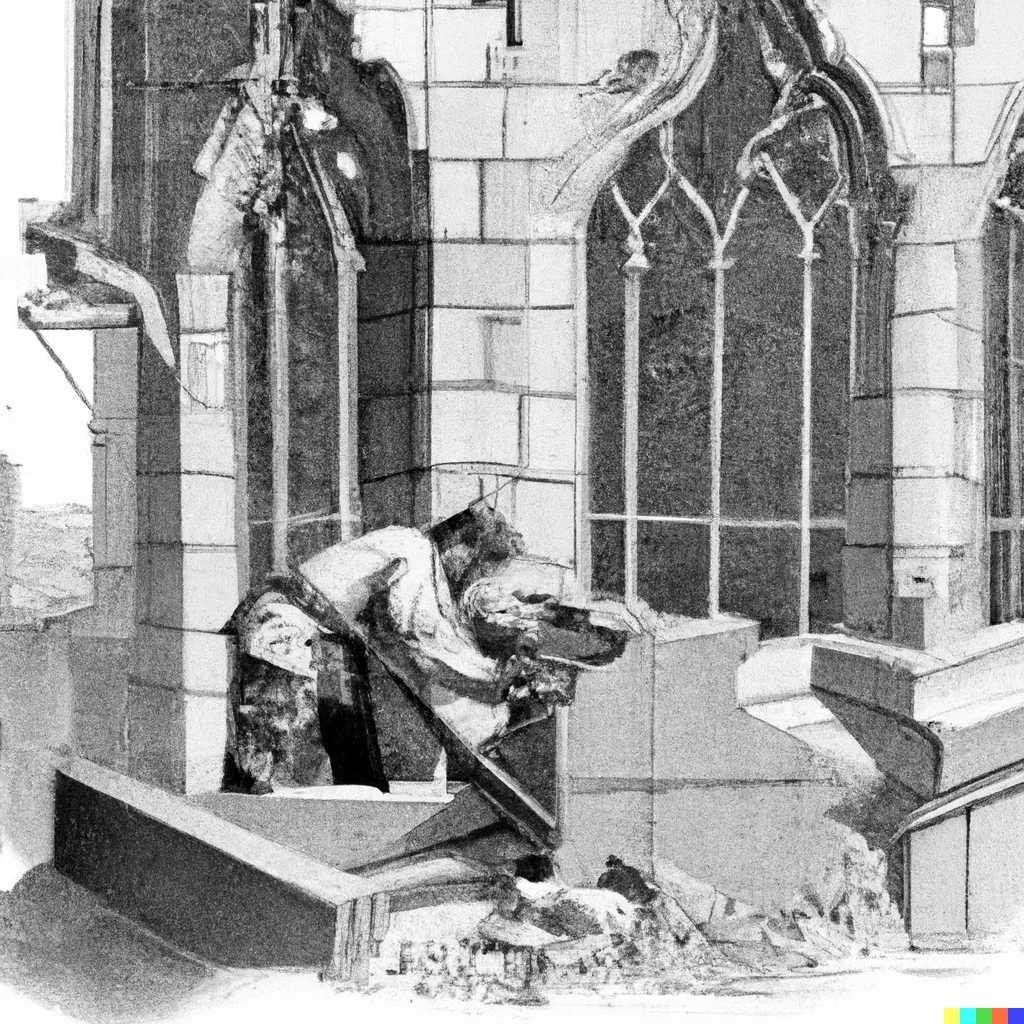
\includegraphics[width=4cm]{image/engraving-of-a-craftman-cutting-a-stone}
        \end{columns}
        \bigbreak
        \flushleft
        1 des 4 règles pour la direction de l'esprit de Descartes~: \textquote{Diviser chacune des difficultés que j'examinerais, en autant de parcelles qu'il se pourrait et qu'il serait requis pour les mieux résoudre.}.
    \end{frame}

    \begin{frame}
        \transdissolve
        \frametitle{Les briques}
        \framesubtitle{3 paradigmes de programmation représentant par des briques\cref{cleanarchitecture}}
        \begin{itemize}
            \item Programmation structurée (sous-ensemble de la programmation impérative), où la brique est le module de code, i.e., des programmes et sous-programmes.
            Il contient les instructions de control de flux (if, else, for, while, etc.).
            \item Programmation orientée objet, où la brique est la classe.
            \item Programmation fonctionnelle, où la brique est la fonction.
        \end{itemize}
        \bigbreak
        La plupart des langages de programmation modernes supportent ces 3 paradigmes, JS, Python, Java, C/C++.
    \end{frame}

    \subsection{Programmation structurée}\label{subsec:briques-struct}
    \begin{frame}
        \transdissolve
        \frametitle{Les briques}
        \framesubtitle{Exemple de programmation structurée}
        Utilisation de tout le control flow classique.
        \bigbreak
        \centering
        \begin{tabular}{cc}
            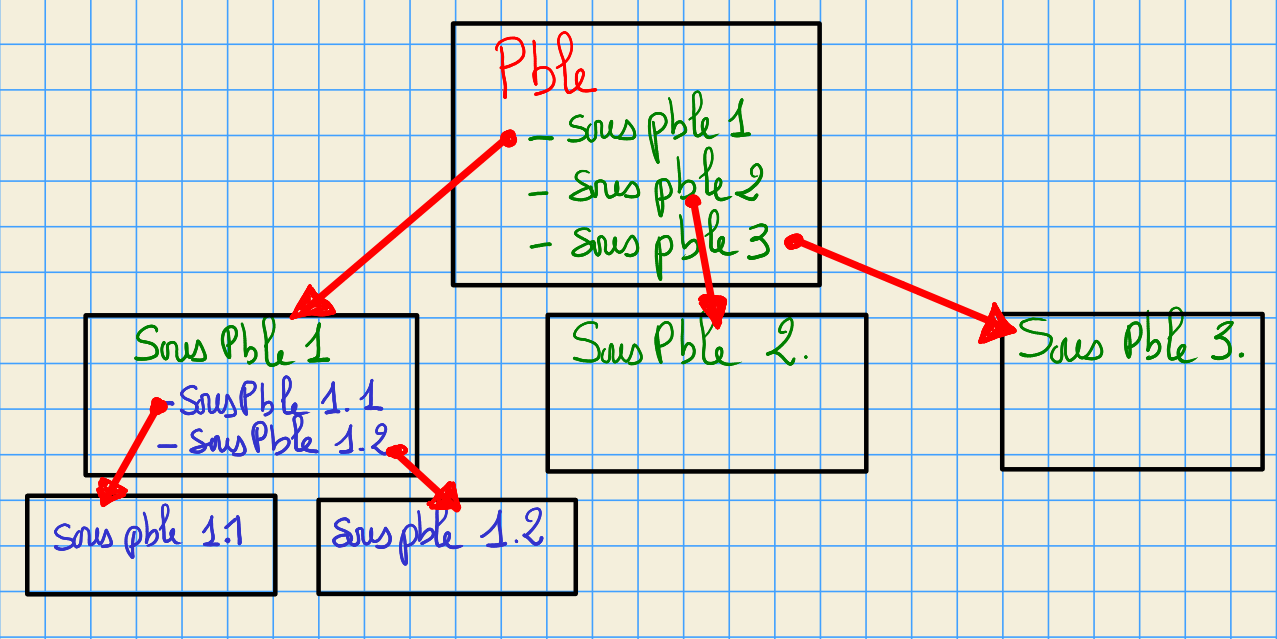
\includegraphics[width=10cm]{image/analyse-topdown-prog-struc}                                                                                                                                        \\
            Analyse top-down pour division des taches en sous-programmes\footnote{Programmation structurée, \url{https://perso.univ-lyon1.fr/marc.buffat/COURS/BOOK_INPROS_HTML/CHAP5/COURS_ALGORITHMIQUE.html}}.                     \\
        \end{tabular}
    \end{frame}

    \subsection{Programmation fonctionnelle}\label{subsec:briques-fonc}
    \begin{frame}[fragile]
        \transdissolve
        \frametitle{Les briques}
        \framesubtitle{Exemple de programmation fonctionnelle\cref{cleanarchitecture}}
        Les briques sont de simples fonctions, des fonctions dîtes pures.
        Les données ne sont modifiées uniquement que par ces fonctions.
        \bigbreak
        Des exemples de langages fonctionnels~: Haskell, Lisp, Erlang, Scala, F\#.
        \bigbreak
        D'autres langages supportent la programmation fonctionnelle comme Python, JS, Java en autres et ont des outils/librairies dédiées à la programmation fonctionnelle.
        Souvent nommées fonctions lambda ou \textquote{arrow functions}, map, reduce, filter, etc.
        \begin{lstlisting}[language=python]
>>> is_even = lambda x: x % 2 == 0 # No return needed?
>>> list(map(is_even, [1, 2, 3, 4]))
[False, True, False, True]
>>> list(filter(is_even, [1, 2, 3, 4])) # Kept only if True
[2, 4]
>>> from functools import reduce
>>> from operator import mul
>>> reduce(mul, [1, 2, 3, 4]) # Function applied to all elements, 1 * 2 * 3 * 4
24
        \end{lstlisting}
    \end{frame}

    \begin{frame}[fragile]
        \transdissolve
        \frametitle{Les briques}
        \framesubtitle{Exemple de programmation fonctionnelle}
        3 modules dédiés à la programmation fonctionnelle dans la \textquote{standard library} Python\footnote{Functional Programming Modules, \url{https://docs.python.org/3/library/functional.html}}~:
        \begin{itemize}
            \item \lstinline{functools}, \textquote{Higher-order functions and operations on callable objects}.
            \item \lstinline{itertools}, \textquote{Functions creating iterators for efficient looping}.
            \item \lstinline{operator}, \textquote{Standard operators as functions}.
        \end{itemize}
        L'équivalent en JS, sans aucune librairie à importer~:
        \begin{lstlisting}[language=java]
> numbers = new Array(1, 2, 3, 4, 5)
[ 1, 2, 3, 4, 5 ]
> const isEven = x => x % 2 === 0;
undefined
> numbers.map(isEven);
[ false, true, false, true, false ]
> numbers.reduce(isEven);
true
> numbers.filter(isEven);
[ 2, 4 ]
> numbers.reduce((x, y) => y * x);
120
        \end{lstlisting}
    \end{frame}

    \subsection{Programmation orientée objet}\label{subsec:briques-oop}
    \begin{frame}[fragile]
        \transdissolve
        \frametitle{Les briques}
        \framesubtitle{Exemple de programmation orientée objet\cref{cleanarchitecture}} (OOP)
        La brique de base en programmation orientée objet est la classe.
        \bigbreak
        En OOP on parle de polymorphisme, c'est la capacité d'un objet, i.e., d'une classe, à prendre plusieurs formes.
        Une évolution dans une classe fille n'implique pas de modification dans la classe mère.
        Une évolution dans une classe mère impacte les classes filles.
        Si ces classes sont dans des modules différents, il n'est même pas nécessaire de recompiler tous les modules.
        Pouvoir controller quelle classe dépend de quelle autre est un atout majeur de cette architecture logicielle.
        \bigbreak
        L'encapsulation des données et des méthodes dans une classe permet un design simple de ce qui appartient à un objet, une instance de classe, et ce qui est accessible depuis l'extérieur.
        \bigbreak
        L'encapsulation et l'héritage qui permet le polymorphisme sont les 2 atouts principaux de la programmation orientée objet.
    \end{frame}

    \begin{frame}[fragile]
        \transdissolve
        \frametitle{Les briques}
        \framesubtitle{Exemple de programmation orientée objet}
        Polymorphisme par héritage d'une classe.
        \begin{lstlisting}
>>> class Oiseau:
        def __init__(self, name):
            self.name = name

>>> class Pigeon(Oiseau):
        def __init__(self, name):
            Oiseau.__init__(self, name)
        def mange_un_filtre_cigarette(self):
            print("{} mange un filtre de cigarette!!!".format(self.name))

>>> class Cygne(Oiseau):
        def __init__(self, name):
            Oiseau.__init__(self, name)
        def plonge(self):
            print("{} plonge dans le lac!!!".format(self.name))

>>> goelan = Oiseau("Jonathan Livingston")
>>> cygne = Cygne("Juste Leblanc") # C'est un Oiseau aussi !
>>> pigeon = Pigeon("Casimir") # Même le pigeaon est un Oiseau !
>>> all(map(lambda x: isinstance(x, Oiseau), [cygne, pigeon, goelan]))
True
        \end{lstlisting}
    \end{frame}

    \begin{frame}[fragile]
        \transdissolve
        \frametitle{Les briques}
        \framesubtitle{Exemple de programmation orientée objet}
        Polymorphisme par héritage d'une classe abstraite.
        \begin{lstlisting}
>>> from abc import ABC, abstractmethod

>>> class Oiseau(ABC): # ABC -> ABstract Class
        def __init__(self):
            pass
        @abstractmethod
        def vole(self): # Polymorphisme au niveau de cette méthode !
            raise NotImplementedError

>>> class Poule(Oiseau):
        def __init__(self):
            Oiseau.__init__(self):
        def vole(self): # Chacun vole à sa manière, son implémentation
            print("Je vole quelques mètres")

>>> cocote = Poule()

>>> cocote.vole()
Je vole quelques mètres
        \end{lstlisting}
    \end{frame}

    \begin{frame}[fragile]
        \transdissolve
        \frametitle{Les briques}
        \framesubtitle{Exemple de programmation orientée objet}
        Contrainte d'implémentation d'une méthode abstraite \lstinline{vole} .

        \begin{lstlisting}
>>> class Dodo(Oiseau):
        def __init__(self):
            Oiseau.__init__(self)

>>> Aussie = Dodo()
---------------------------------------------------------------------------
TypeError                                 Traceback (most recent call last)
Cell In [10], line 1
----> 1 Aussie = Dodo()

TypeError: Can't instantiate abstract class Dodo with abstract method vole
        \end{lstlisting}
    \end{frame}

    \subsection{Exercice}\label{subsec:briques-exe}
    \begin{frame}
        \transdissolve
        \frametitle{Les types de briques}
        \framesubtitle{Exercice \execcounterdispinc{} de 5 minutes}
        Trouver quel type de paradigme de programmation est utilisé dans les exemples suivants~:
        \begin{itemize}
            \item \url{https://github.com/facebook/Haxl/}
            \item \url{https://github.com/gurupratap-matharu/Bike-Rental-System/blob/master/main.py}
            \item \url{https://github.com/papit-fr/fsma/}
        \end{itemize}
        Tirage au sort d'un étudiant pour chaque exemple, il doit expliquer pourquoi il pense que c'est ce type de programmation.
    \end{frame}


    \section{TDD}

    \begin{frame}
        \transdissolve
        \frametitle{Le TDD}
        \framesubtitle{Test Driven Development}
        Vouloir aller plus vite sans faire de test semble être une mauvaise idée.

        Ce qui pratiquent le TDD vont plus vite dès le début d'un projet\cref{cleanarchitecture}~!

        Entre autre, les tests unitaires font réduire la taille des classes, functions et des méthodes, ce qui améliore architecture.
        \bigbreak
        \centering
        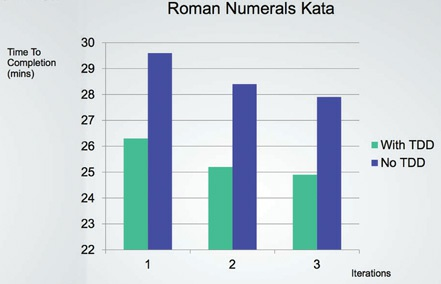
\includegraphics[width=8cm]{image/tdd-vs-no-tdd}
    \end{frame}

    \begin{frame}
        \transdissolve
        \frametitle{Le TDD}
        \framesubtitle{Quel type(s) de test~?}
        Tous les types de tests possibles sont à écrire dès que possible avant même de commencer à coder.
        Les tests unitaires sont en général les plus simples à écrire et les plus rapides à exécuter.
        \bigbreak
        Les éléments centraux, les règles de gestions, les \textquote{business rules} doivent être testables sans les éléments périphériques\cref{cleanarchitecture}~:
        \bigbreak
        \centering
        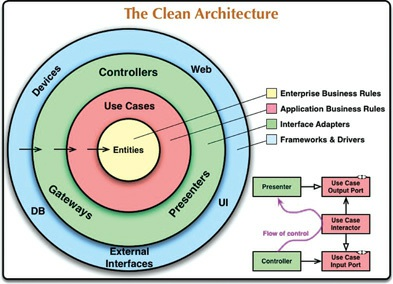
\includegraphics[width=6cm]{image/the-clean-architecture}
    \end{frame}

    \begin{frame}
        \transdissolve
        \frametitle{Le TDD}
        \framesubtitle{Quel types de test~?}
        Edsger Dijkstra~: \textquote{Testing shows the presence, not the absence of bugs.}
        \bigbreak
        \begin{columns}
            \column{0.5\textwidth}
            Autrement dit, l'univers des tests est infini, on n'a jamais la certitude de suffisamment tester.
            \bigbreak
            Même le coverage est une mauvaise mesure.
            \column{0.5\textwidth}
            \centering
            
\includegraphics[width=5cm]{image/monk-looking-the-deepness-of-the-stars-in-the-night-sky}
        \end{columns}
    \end{frame}

    \begin{frame}
        \transdissolve
        \frametitle{Le TDD}
        \framesubtitle{Exercices \execcounterdispinc{}}
        De nombreux exercices de TDD sont disponibles sur le web comme par sur GitHub, \url{https://github.com/gabbloquet/entrainement-au-tdd}.
        \bigbreak
        En 30 minutes, sans assistant du type ChatGPT, réaliser l'un des plus classique d'entre eux, le \textquote{FizzBuzz}, \url{https://github.com/gabbloquet/entrainement-au-tdd/tree/master/src/main/java/io/github/gabbloquet/tddtraining/FizzBuzz}~.
        Respecter l'esprit du TDD qui veut que l'on écrive les tests avant le code~:
        \begin{enumerate}
            \item Écrire un test par requirement.
            \item Écrire l'algorithme.
            \item Refactoriser.
            \item Revenir à l'étape 2 jusqu'à ce que tous les test passent.
        \end{enumerate}

    \end{frame}


    \section{Les mesures}\label{sec:les-mesures}

    \begin{frame}
        \transdissolve
        \frametitle{Les mesures du couplage}
        \framesubtitle{L'importance des données}
        L'architecture c'est le monde du compromis, des possibilités infinies.
        \bigbreak
        L'intuition, l'expérience, les connaissances et le bon sens, nous guiderons.

        Mais il est possible de qualifier l'architecture avec des mesures et donc d'avoir une approche \textquote{Data Driven} .
        \bigbreak
        Nous verrons dans cette section les différentes des métriques classiques, mais pas toutes, car elles sont nombreuses.

        On parle parfois aussi des CK (Chidamber \& Kemerer) metrics qui peuvent ressembler, etc.
    \end{frame}

    \begin{frame}
        \transdissolve
        \frametitle{Les mesures du couplage}
        \framesubtitle{L'\textquote{abstractness} $A$\cref{fundsofsoftarch}}
        L'\textquote{abstractness}  une mesure de l'abstraction par rapport aux implémentations concrètes.
        Elle fut introduite par Robert C. Martin.
        \begin{equation}
            A = \frac{\sum Ca}{\sum Cc}
        \end{equation}
        Dans l'équation 1~:
        \begin{itemize}
            \item $A$ est \textquote{abstractness}.
            \item $Ca$ est le nombre de classe(s) abstraite(s).
            \item $Cc$ est le nombre de classe(s) concrète(s).
        \end{itemize}
        \bigbreak
        Les valeurs de $A$ sont entre 0 et 1.
        Les extrêmes proches de 0 ou 1 sont à éviter, elles représentent des architectures trop concrètes ou trop abstraites.
    \end{frame}

    \begin{frame}
        \transdissolve
        \frametitle{Les mesures du couplage}
        \framesubtitle{Couplage afférent}
        Le couplage afférent est le nombre total de classe(s) qui dépend(ent) de la classe A~:
        \bigbreak
        \centering
        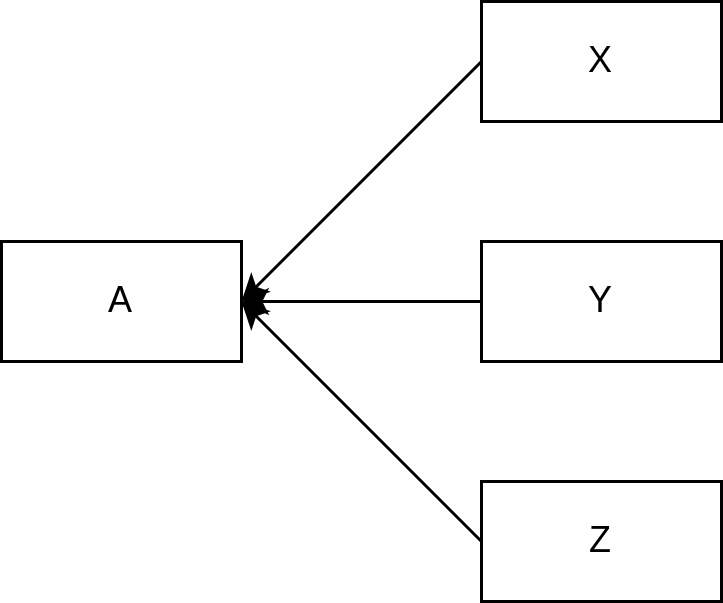
\includegraphics[width=5cm]{image/afferent-coupling.drawio}
        \bigbreak
        \flushleft
        Ici $Ca$ est 3.

        Un $Ca$ élevé impacte principalement la portabilité.
        Car ce code viendra forcément avec beaucoup de code en dépendance.
    \end{frame}

    \begin{frame}
        \transdissolve
        \frametitle{Les mesures du couplage}
        \framesubtitle{Couplage efférent $Ce$}
        Le couplage efférent est le nombre total de classe(s) dont dépend la classe A~:
        \bigbreak
        \centering
        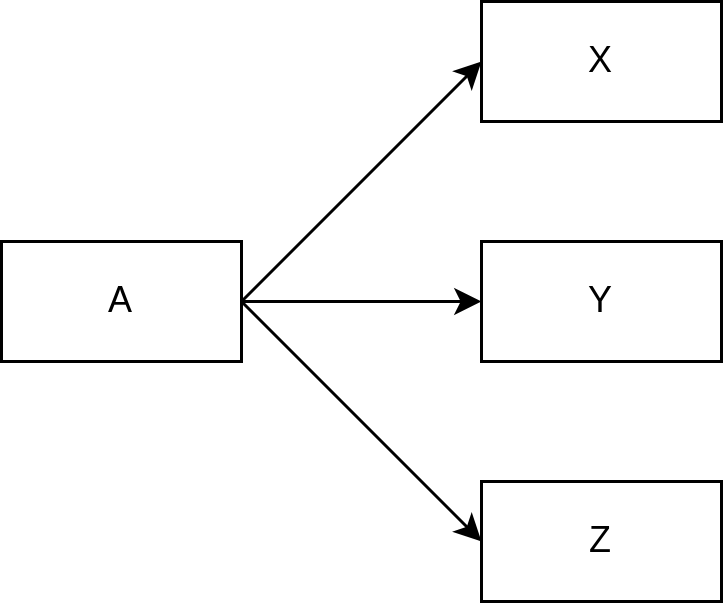
\includegraphics[width=5cm]{image/efferent-coupling.drawio}
        \bigbreak
        \flushleft
        Ici $Ce$ est 3.

        Plus le $Ce$ est élevé, plus le code est difficile à reuse et à maintenir.
    \end{frame}

    \begin{frame}
        \transdissolve
        \frametitle{Les mesures du couplage}
        \framesubtitle{L'\textquote{instability} $I$\cref{fundsofsoftarch}}
        L'\textquote{instability} est une autre mesure qui en découle.
        Elle détermine la volatilité du code, l'effort à fournir pour modifier une partie du code sans devoir en modifier une autre.
        \begin{equation}
            I = \frac{Ce}{Ce + Ca}
        \end{equation}
        Dans l'équation 2~:
        \begin{itemize}
            \item $I$ est \textquote{instability}
            \item $Ca$ couplage afférent, objet ou package en entrée (\textquote{a} en premier d'où \textquote{entrée}).
            \item $Ce$ couplage efférent, objet ou package en sortie (\textquote{e} comme \textquote{exit}).
        \end{itemize}
        \bigbreak
        Quand elle est trop élevée, qu'elle tend vers 1, le code casse vite à cause d'un fort couplage.
        Elle a donc un impact négatif sur le reuse, les correctifs, la maintenance et la portabilité.
    \end{frame}

    \begin{frame}
        \transdissolve
        \frametitle{Les mesures du couplage}
        \framesubtitle{La\textquote{Distance from main sequence} $D$\cref{fundsofsoftarch}\footnotestep\footnote{A Study on Robert C.Martin’s Metrics for Packet Categorization
        Using Fuzzy Logic, Gurpreet Kaur and Deepak Sharma\url{https://gvpress.com/journals/IJHIT/vol8_no12/15.pdf}}}
        Une cinquième métrique introduite par Robert C. Martin est la \textquote{Distance from main sequence}.
        \bigbreak
        Elle définit une relation entre $A$ et $I$ comme suit~:
        \begin{columns}
            \column{0.5\textwidth}
            \begin{equation}
                D = |A + I - 1|
            \end{equation}
            \column{0.5\textwidth}
            \centering
            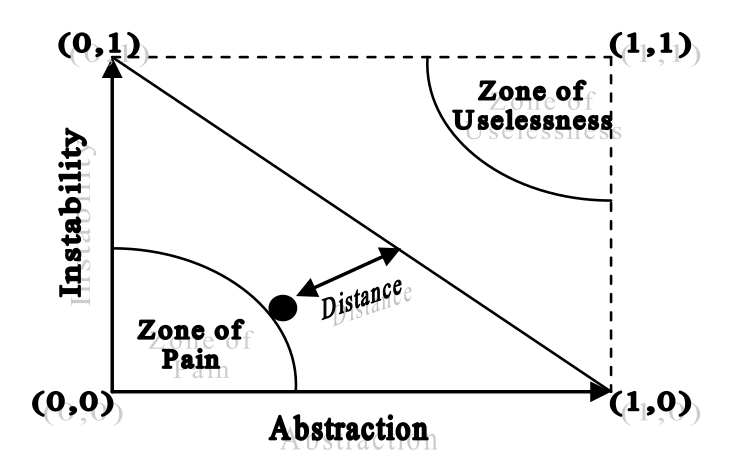
\includegraphics[width=5cm]{image/distance-from-main-sequence}
        \end{columns}
        \flushleft
        $D$ doit s'approcher de 0 pour une architecture souhaitable.
        Si $D$ est élevé, on s'éloigne de compromis acceptable.
    \end{frame}

    \begin{frame}
        \transdissolve
        \frametitle{Les mesures du couplage}
        \framesubtitle{Exercice \execcounterdispinc{} de 30 minutes}
        Calculer les valeurs de $Ca$, $Ce$, $A$, $I$ et $D$ pour chaque classe du source \url{https://github.com/St-Michel-IT/architecture-application/blob/main/coupling.py}.
        \bigbreak
        Restituer le résultat dans un tableau Excel et un graphique avec les $D$ et la droite \textquote{main sequence}.
    \end{frame}

    \begin{frame}
        \transdissolve
        \frametitle{Les mesures du couplage}
        \framesubtitle{Résultat de l'exercice précédent}
        \centering
        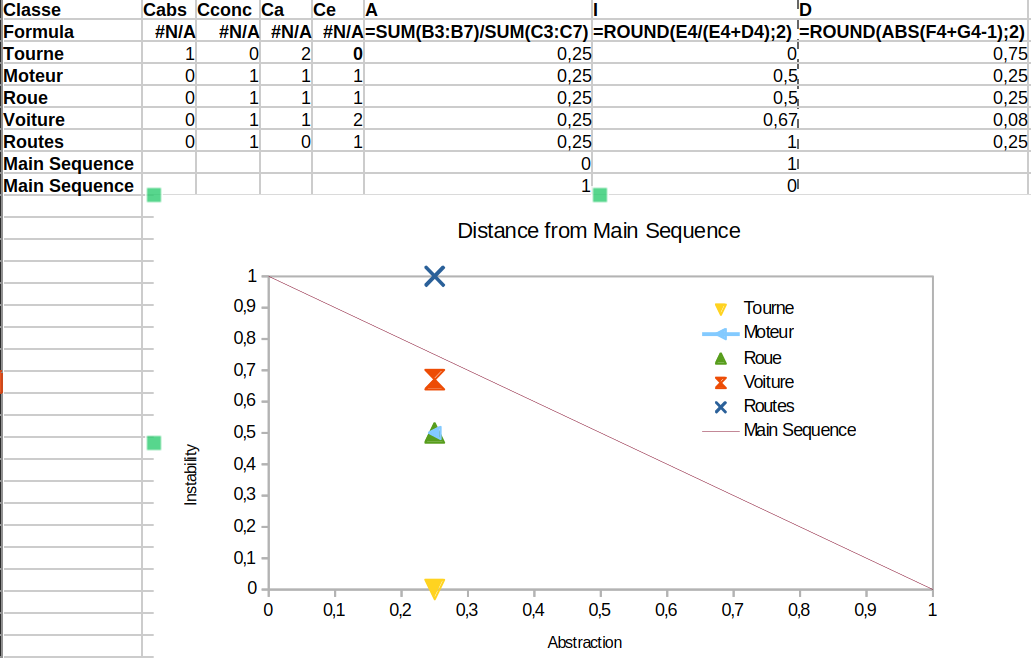
\includegraphics[width=10cm]{image/exercice-metrics-1}
    \end{frame}

    \begin{frame}[fragile]
        \transdissolve
        \frametitle{Les mesures du couplage}
        \framesubtitle{Les outils}
        Certains outils comme \lstinline{JCAT}\footnote{Tool for Measuring Coupling in Object-Oriented Java Software, \url{https://shorturl.at/npDR2}} en Java ou \lstinline{module_coupling_metrics}\footnote{\url{https://github.com/Oaz/module_coupling_metrics}} en Python permettent de calculer ces métriques.
        % shell listing with the command~:
        \begin{lstlisting}[language=bash]
$ module_coupling_metrics data_management.py
        \end{lstlisting}
        \begin{columns}
            \column{0.5\textwidth}
            \centering
            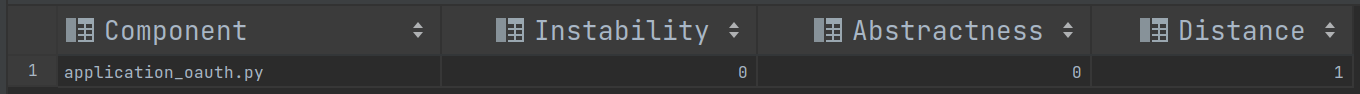
\includegraphics[width=5cm]{image/data-management-metrics-table}
            \column{0.5\textwidth}
            \centering
            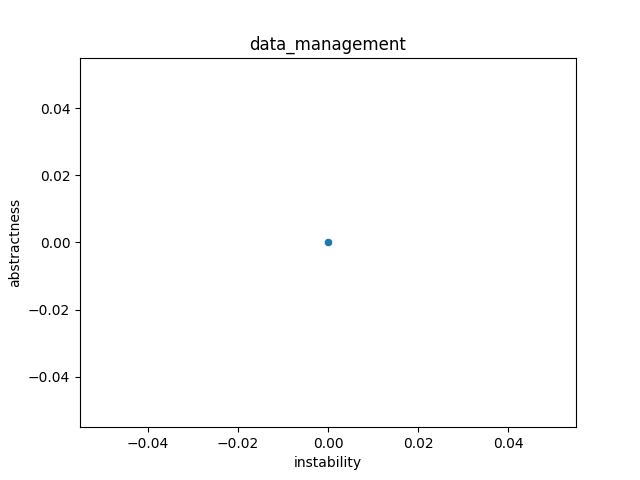
\includegraphics[width=5cm]{image/data-management-disance-chart}
        \end{columns}

        Attention à bien comprendre ces métriques et comment les interpréter.
        \lstinline{module_coupling_metrics} ne calcule le couplage qu'entre modules.
        \bigbreak
    \end{frame}

    \begin{frame}
        \transdissolve
        \frametitle{Les mesures de la complexité cyclomatique}
        \framesubtitle{La théorie}
        Établie en 1976, elle est devenue le standard de mesure de complexité du code.
        \bigbreak
        Elle se calcule pour une méthode ou fonction avec l'équation suivante~:
        \begin{equation}
            CC = E - N + 2
        \end{equation}
        Où~:
        \begin{itemize}
            \item $CC$ est la complexité cyclomatique.
            \item $E$ comme \textquote{edge} , est le nombre d'arêtes (les \lstinline{return} , \lstinline{yield}, \lstinline{exit}) du graphe de contrôle de flux.
            \item $N$ comme \textquote{node} , est le nombre de nœuds, les \lstinline{if}, \lstinline{while}, \lstinline{for}, du graphe de contrôle de flux.
        \end{itemize}
        \bigbreak
        Les valeurs au-dessous de 5 sont bonnes, au-dessus de 10 il y a danger\cref{fundsofsoftarch} .
        \bigbreak
        Une $CC$ trop élevée est un code smell de Sonar Qube.
    \end{frame}

    \begin{frame}[fragile]
        \transdissolve
        \frametitle{Les mesures de la complexité cyclomatique}
        \framesubtitle{Exemple de fonction}
        % C code listing
        \begin{lstlisting}[language=c]
uint64_t fsma(uint64_t base, uint64_t exp, uint64_t mod) {
    uint64_t res = 1;
    while (exp > 1) {
        // If the exponent digit is 1, then multiply
        if (exp & 1) {
            res = (res * base) % mod;
            // If an intermediate result is zero, we can return 0.
            // The result will be zero anyway
            if (res == 0) {
                return 0;
            }
        }
        // If the exponent digit is 0, then square
        base = (base * base) % mod;
        exp >>= 1;
    }
    return (base * res) % mod;
}
        \end{lstlisting}

        Ici $E$ est 2 et $N$ est 3, donc $CC$ est 1.
    \end{frame}

    \begin{frame}[fragile]
        \transdissolve
        \frametitle{Les mesures de la complexité cyclomatique}
        \framesubtitle{Exercice \execcounterdispinc{}}
        \begin{columns}
            \column{0.5\textwidth}
            Cette métrique peut se calculer plus facilement avec un graphe de contrôle de flux.
            \bigbreak
            Calculer la complexité cyclomatique de la fonction décrite à droite.
            \column{0.5\textwidth}
            \centering
            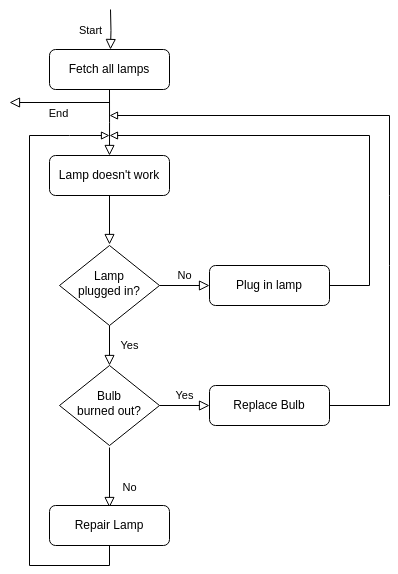
\includegraphics[width=5cm]{image/flux-diagram.drawio}
        \end{columns}
    \end{frame}

    \begin{frame}[fragile]
        \transdissolve
        \frametitle{Les mesures de la complexité cyclomatique}
        \framesubtitle{Exercice \execcounterdispinc{}}
        Calculer la complexité cyclomatique des fonctions de l'implémentation de l'algorithme de hachage MD5 du noyau Linux.
        \bigbreak
        Le code est sur Github~: \url{https://github.com/torvalds/linux/blob/master/crypto/md5.c}
        \bigbreak
        Rendre un tableau des valeurs de $CC$ pour chaque fonction et en tirer une conclusion.
    \end{frame}


    \section{Mid-level architecture}\label{sec:mid-level-architecture}

    \subsection{Généralités}\label{subsec:mid-level-generalites}

    \begin{frame}
        \transdissolve
        \frametitle{\textquote{Mid-level} architecture}
        \framesubtitle{Comment agencer les briques}
        Les briques vues précédemment sont nécessaires mais pas suffisantes pour construire un système.
        Si elles ne sont pas correctement conçues il est inutile de les intégrer à un design élaboré, le système risque fortement de ne pas fonctionner
        \bigbreak
        Pour qu'un système fonctionne, il faut que les briques soient correctement agencées.
        C'est la \textquote{mid-level architecture}.
        \bigbreak
        De nombreux principes ou patterns existent pour agencer les briques.
        Comme par exemple~:
        \begin{itemize}
            \item \textbf{SOLID}~: Single Responsibility, Open-Closed, Liskov Substitution, Interface Segregation, Dependency Inversion.
            \item \textbf{Hexagonal Architecture}~: A.K.A Ports and Adapters.
            \item \textbf{Onion Architecture}~: Une couche intérieur ne sait rien de celle plus extérieur.
            \item Many more\ldots
        \end{itemize}
    \end{frame}

    \begin{frame}
        \transdissolve
        \frametitle{\textquote{Mid-level} architecture}
        \framesubtitle{Comment agencer les briques}
        De manière générale ces différents patterns ne sont pas concurrents.
        Ils ne se contredisent pas.
        Ils peuvent même être utilisés ensemble.
        \bigbreak
        La coexistence des ces patterns permet de visualiser un même problème sous différents point de vue\cref{cleanarchitecture}\footnotestep\footnote{The Onion Architecture : part 1, \url{https://jeffreypalermo.com/2008/07/the-onion-architecture-part-1/}}~:
        \begin{columns}
            \column{0.5\textwidth}
            \centering
            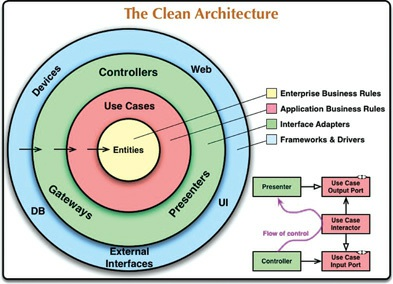
\includegraphics[width=5cm]{image/the-clean-architecture}
            \column{0.5\textwidth}
            \centering
            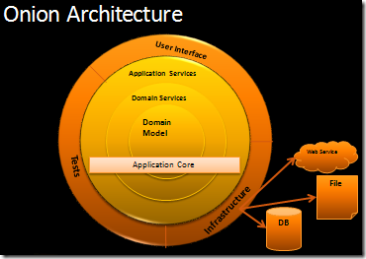
\includegraphics[width=5cm]{image/onion-architecture}
        \end{columns}
    \end{frame}

    \begin{frame}
        \transdissolve
        \frametitle{\textquote{Mid-level} architecture}
        \framesubtitle{Comment agencer les briques}
        De même, l'architecture hexagonale semble similaire elle aussi\cref{cleanarchitecture}\footnotestep\footnote{Architecture hexagonale, Wikipédia, \url{https://fr.wikipedia.org/wiki/Architecture_hexagonale}}~:
        \bigbreak
        \begin{columns}
            \column{0.5\textwidth}
            \centering
            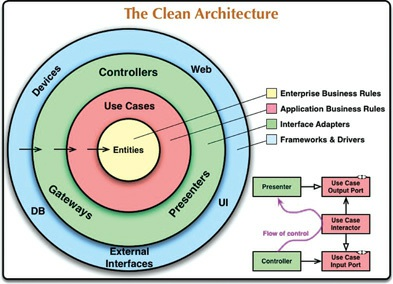
\includegraphics[width=5cm]{image/the-clean-architecture}
            \column{0.5\textwidth}
            \centering
            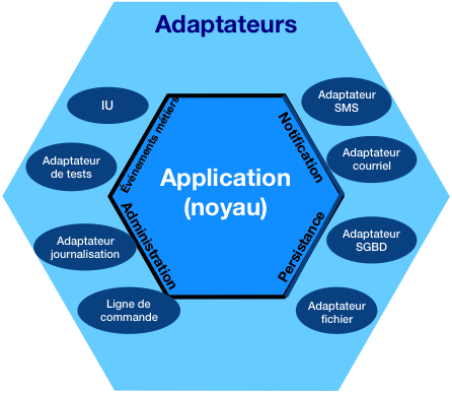
\includegraphics[width=5cm]{image/hexagonal-architecture}
        \end{columns}
    \end{frame}

    \subsection{S.O.L.I.D}\label{subsec:mid-level-solid}


    \begin{frame}
        \transdissolve
        \frametitle{Les principes S.O.L.I.D}
        \framesubtitle{Histoire et définition\cref{cleanarchitecture}}
        Démarrés dans les années 80, ils sont finalisés en 2004 par Robert C. Martin.
        S.O.L.I.D est un acronyme pour 5 principes de design.
        \bigbreak
        Les buts de ces principes sont~:
        \begin{itemize}
            \item Tolérer le changement.
            \item Être facile à comprendre.
            \item Ils sont les composants de base qui peuvent être utilisés dans tout logiciel.
        \end{itemize}
        \bigbreak
        C'est de la \textquote{Mid-level architecture}, car même avec des briques biens conçues, agencées selon ces principes, il manque encore l'architecture de plus haut niveau.
    \end{frame}

    \begin{frame}
        \transdissolve
        \frametitle{Les principes S.O.L.I.D}
        \framesubtitle{Les 5 principes résumés\cref{cleanarchitecture}}
        \begin{footnotesize}
            \begin{itemize}
                \item \textbf{Single Responsibility Principle}~: Une classe ne doit avoir qu'une seule responsabilité.
                \item \textbf{Open-Closed Principle}~: Une classe doit être ouverte à l'extension mais fermée à la modification.
                \item \textbf{Liskov Substitution Principle}~: Une instance de type T doit pouvoir être remplacée par une instance de type G, tel que G sous-type de T, sans que cela ne modifie la cohérence du programme.
                Cela garantit que les sous-classes peuvent être utilisées de manière interchangeable avec leurs classes de base.
                \item \textbf{Interface Segregation Principle}~: Les classes ne doivent pas être forcés d'implémenter des interfaces qu'ils n'utilisent pas.
                Préférer plusieurs interfaces spécifiques pour chaque client plutôt qu'une seule interface générale.
                Cela évite aux classes de dépendre de méthodes dont elles n'ont pas besoin, réduisant ainsi les couplages inutiles.
                \item \textbf{Dependency Inversion Principle}~: Il faut dépendre des abstractions, pas des implémentations.
                Cela favorise la modularité, la flexibilité et la réutilisabilité en réduisant les dépendances directes entre les modules.
                Le code des règles de haut-niveau ne doit pas dépendre du code de détail bas-niveau.
                Mais les détails peuvent dépendre des règles haut-niveau.
            \end{itemize}
        \end{footnotesize}
    \end{frame}

    \subsection{Single Responsibility Principle}\label{subsec:mid-level-s}

    \begin{frame}
        \transdissolve
        \frametitle{Single Responsibility Principle (SRP)}
        \framesubtitle{Définition\cref{cleanarchitecture}}
        \begin{dangercolorbox}
            Ne pas confondre avec le refactor d'une méthode ou d'une fonction en méthode ou fonction plus atomique.
        \end{dangercolorbox}
        Selon Robert C. Martin, \textquote{A module should be responsible to one, and only one, actor}.
        \begin{columns}
            \column{0.5\textwidth}
            Module est souvent synonyme de fichier source.

            Donc autrement dit, dans un fichier source, on trouve les fonctions ou les structures de données responsables face à un seul acteur.
            \column{0.5\textwidth}
            \centering
            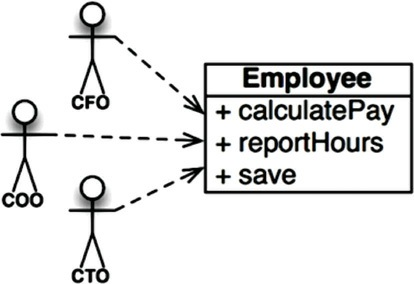
\includegraphics[width=5cm]{image/s-to-avoid} \\ A éviter \\
        \end{columns}
    \end{frame}

    \begin{frame}
        \transdissolve
        \frametitle{Single Responsibility Principle}
        \framesubtitle{Exercice \execcounterdispinc{} de 15 minutes}
        \begin{columns}
            \column{0.5\textwidth}
            Quelles solutions pour éviter ce pattern anti-SRP~?
            \bigbreak
            \column{0.5\textwidth}
            \centering
            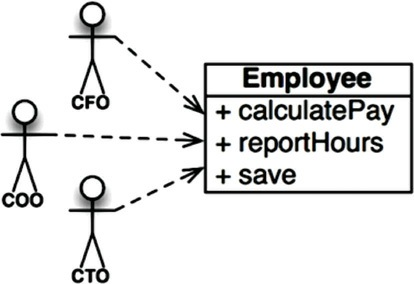
\includegraphics[width=5cm]{image/s-to-avoid}
        \end{columns}
        \flushleft
        Les exigences~:
        \begin{itemize}
            \item Refactoriser des fonctions \lstinline{calculatePay}, \lstinline{reportHours} et \lstinline{save} avec le(s) éventuel(s) argument(s) nécessaire(s) pour qu'elles respectent le SRP~.
            \item Ajouter les attribues nécessaire(s) et au moins 4 méthodes à la classe \lstinline{Employee} tout en respectant le SRP~.
            \item Répondre sous forme d'un schéma (en utilisant Draw.io par exemple) avec les différents et classe(s), méthodes.
        \end{itemize}
    \end{frame}

    \begin{frame}
        \transdissolve
        \frametitle{Single Responsibility Principle}
        \framesubtitle{Exercice \execcounterdispinc{} de 30 minutes}
        Coder la solution de manière simpliste.
        \bigbreak
        Appliquer le TDD, rédiger les tests unitaires avant de coder.
        \bigbreak
        A quoi resemble l'arborescence du projet~?
        \bigbreak
        Commiter dans un dépôt Git, le schéma issu de l'exercice précédent, le code et les tests.
        \bigbreak
        Le travail de certains étudiants sera évalué.
        \bigbreak
        \centering
        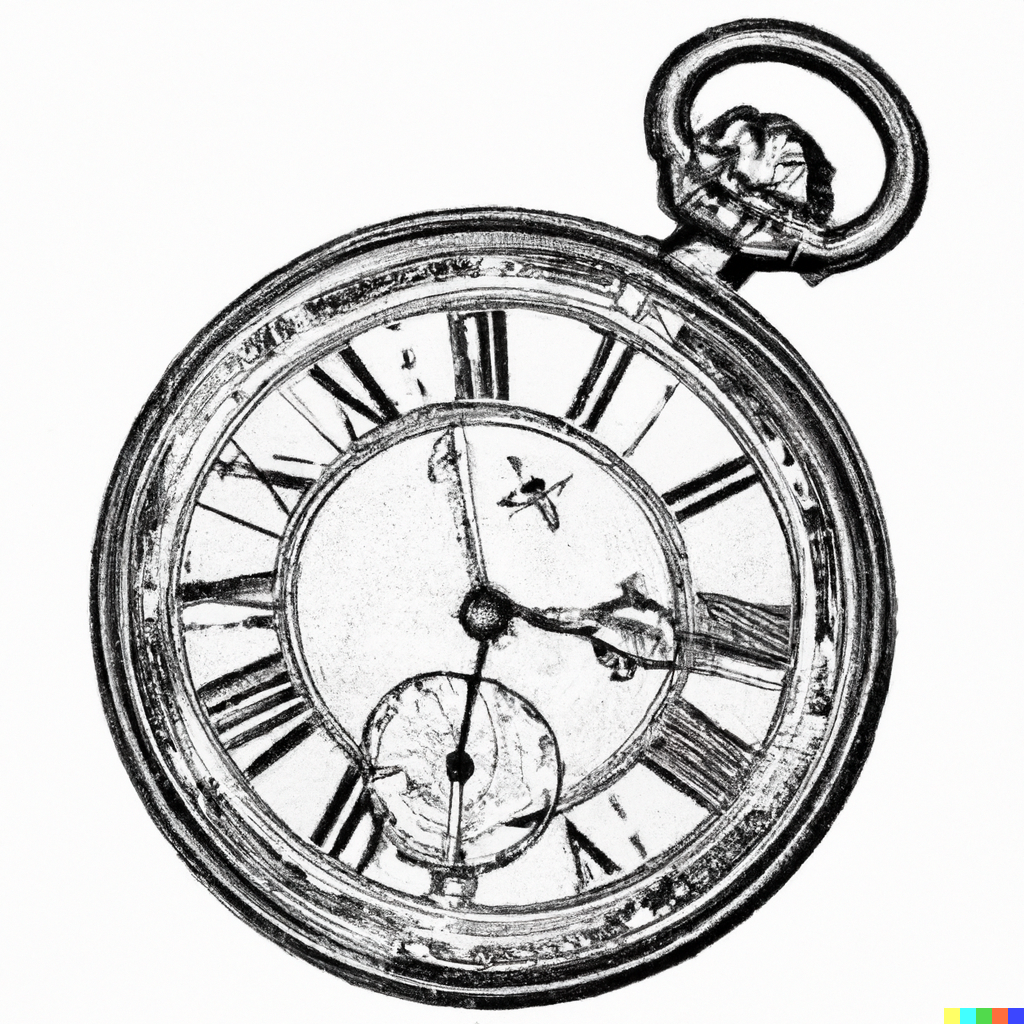
\includegraphics[width=3cm]{image/engraving-of-an-old-watch}
    \end{frame}

    \subsection{Open-Closed Principle}\label{subsec:mid-level-o}

    \begin{frame}
        \transdissolve
        \frametitle{Open-Closed Principle (OCP)}
        \framesubtitle{Définition\cref{cleanarchitecture}}
        OCP veut dire~: \textquote{A software artifact should be open for extension but closed for modification}.
        \bigbreak
        En d'autres termes, un code doit être extensible, on peut ajouter du code et des fonctionnalités sans modifier le code existant.
        Encore une fois, cela permet de tolérer le changement en limitant les risques de bug et en facilitant la maintenance.
        \bigbreak
        Une des solutions est de séparer tout ce qui est susceptible de changer pour des raisons différentes dans le futur.
    \end{frame}

    \begin{frame}
        \transdissolve
        \frametitle{Open-Closed Principle}
        \framesubtitle{Exercice \execcounterdispinc{} de 30 minutes}
        Refactoriser le code \url{https://github.com/St-Michel-IT/architecture-application/blob/main/open-close-bank-customer.py}.
        Le code souhaité doit être extensible sans modification pour pouvoir retourner les informations actuellement printées dans stdout en HTML~.
        \begin{columns}
            \column{0.5\textwidth}
            Appliquer le TDD, rédigez les tests unitaires avant de coder.
            \bigbreak
            Commiter dans un dépôt Git, le schéma issu de l'exercice précédent, le code et les tests.
            \bigbreak
            Le travail de certains étudiants sera évalué.
            \column{0.5\textwidth}
            \centering
            \centering
            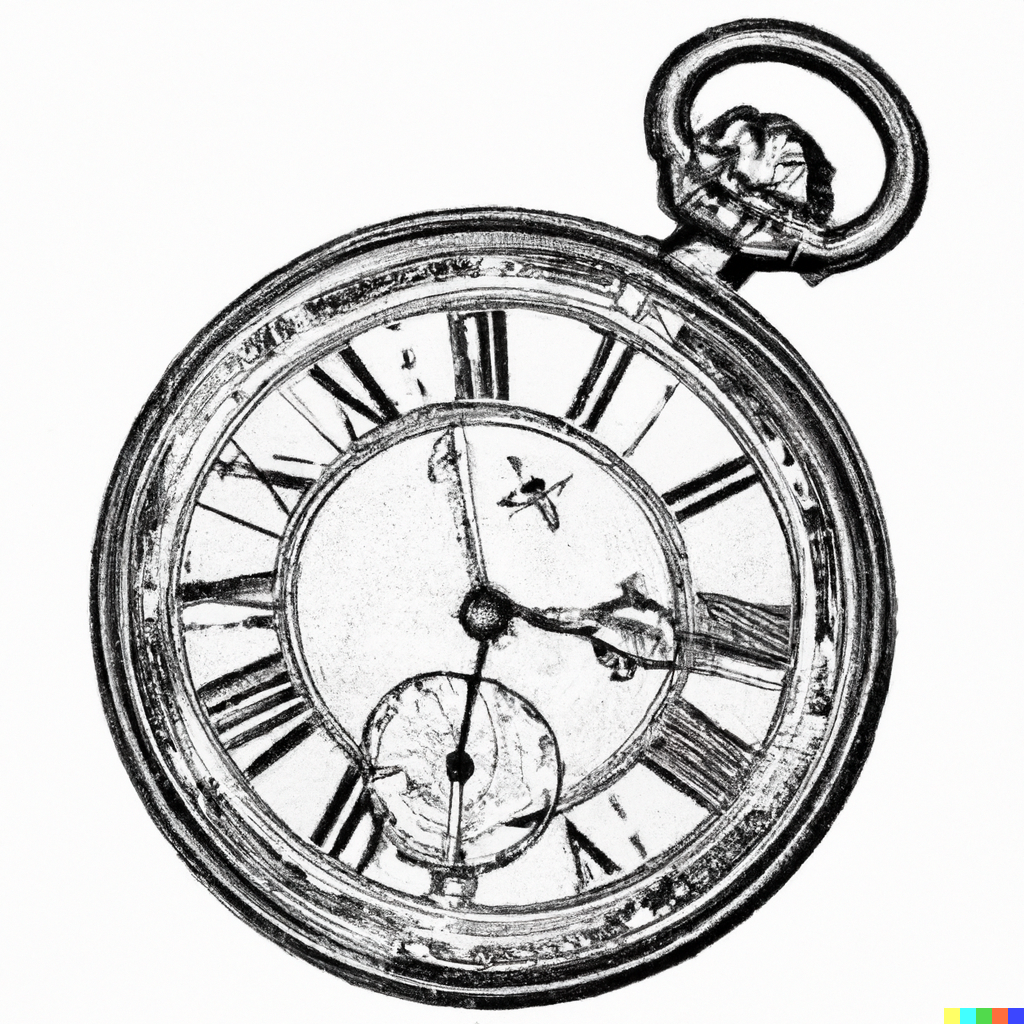
\includegraphics[width=3cm]{image/engraving-of-an-old-watch}
        \end{columns}
    \end{frame}

    \begin{frame}[fragile]
        \transdissolve
        \frametitle{Open-Closed Principle}
        \framesubtitle{Exercice \execcounterdispinc{} de 30 minutes avec les interfaces}
        En Java comme dans beaucoup de language il existe des interfaces.
        Pour rappel, une interface est une structure, une liste de méthodes que les classes qui l'implémentent doivent respecter.
        Comme les classes abstraites, une implementation, i.e., une classe en hérite.
        Elles ne peuvent pas être instanciée directement.
        \begin{lstlisting}[language=java]
public class UserAgeValidator {
  public boolean isOldEnoughToDrinkAlcohol(int age) {
    return age >= 18;
  }
}
        \end{lstlisting}
        Cette classe ne respecte pas le OCP, si on l'applique à plusieurs pays.
        \begin{lstlisting}[language=java]
public class UserAgeValidator {
  public boolean isOldEnoughToDrinkAlcohol(int age, String stateCode) {
    return stateCode.equalsIgnoreCase('FR') && age >= 18
      || stateCode.equalsIgnoreCase('US') && age >= 21
  }
}
        \end{lstlisting}
    \end{frame}

    \begin{frame}
        \transdissolve
        \frametitle{Open-Closed Principle}
        \framesubtitle{Exercice \execcounterdispinc{} de 30 minutes avec les interfaces}
        En utilisant les interfaces, refactoriser la classe \lstinline{UserAgeValidator} pour qu'elle respecte le OCP et créer les classes qui l'implémentent pour divers pays.
        \bigbreak
        \begin{columns}
            \column{0.5\textwidth}
            Commiter dans un dépôt Git, le schéma issu de l'exercice précédent, le code et les tests.
            \bigbreak
            Le travail de certains étudiants sera évalué.
            \column{0.5\textwidth}
            \centering
            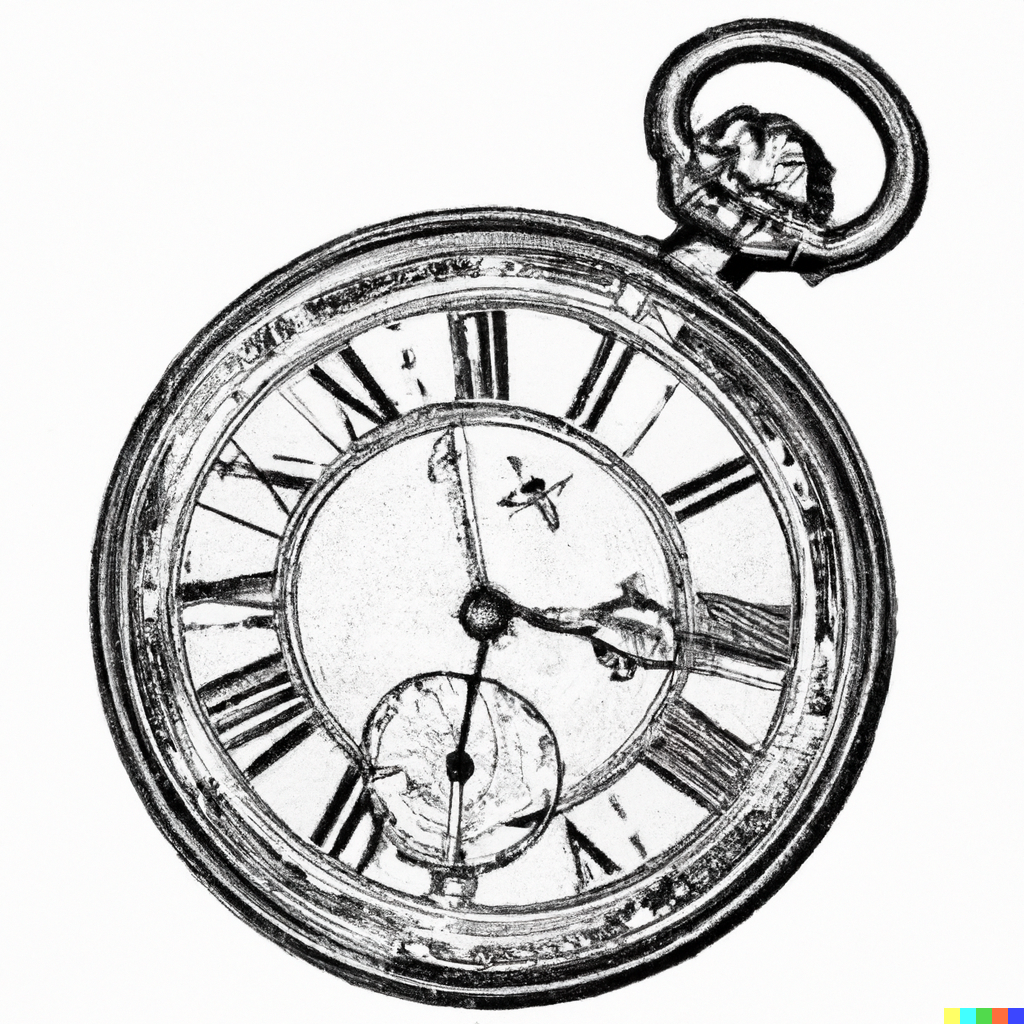
\includegraphics[width=3cm]{image/engraving-of-an-old-watch}
        \end{columns}
    \end{frame}

    \begin{frame}[fragile]
        \transdissolve
        \frametitle{Liskov Principle}
        \framesubtitle{Définition\cref{cleanarchitecture}}
        Une classe enfant doit pouvoir être utilisée à la place de sa classe mère sans que cela ne modifie le comportement du programme.
        \bigbreak
        Pour rappel, évidemment, une classe enfant peut être substitué par un autre enfant de la même classe mère.
        \bigbreak
        Autrement dit une classe fille ne doit pas casser pas le code de la classe mère.
        Ne jamais surcharger une méthode de la classe mère.
        % Python listing
        \begin{lstlisting}[basicstyle=\ttfamily\tiny]]
# EXEMPLE À NE PAS SUIVRE !!!
class Bird:
    def fly(self):
        pass

class Ostrich(Bird):
    def fly(self):
        raise NotImplementedError("Ostriches cannot fly!")

bird = Bird()
bird.fly()  # Output: (no implementation)

ostrich = Ostrich()
ostrich.fly()  # Raises NotImplementedError
        \end{lstlisting}
    \end{frame}

    \begin{frame}
        \transdissolve
        \frametitle{Liskov Principle}
        \framesubtitle{Exercice \execcounterdispinc{} de refactoring de 15 minutes}
        Refactoriser le code \url{https://github.com/St-Michel-IT/architecture-application/blob/main/liskov-rectangle.py}.
        La fonction \lstinline{use_it} ne peut pas être utilisée avec la classe \lstinline{Square} sans modification.
        Refactoriser cette dernière pour qu'elle le puisse et donc qu'elle respecte le Liskov Principle.
        \bigbreak
        \begin{columns}
            \column{0.5\textwidth}
            Appliquer le TDD, rédiger les tests unitaires avant de coder.
            \bigbreak
            Commiter dans un dépôt Git, le schéma issu de l'exercice précédent, le code et les tests.
            \bigbreak
            Le travail de certains étudiants sera évalué.
            \column{0.5\textwidth}
            \centering
            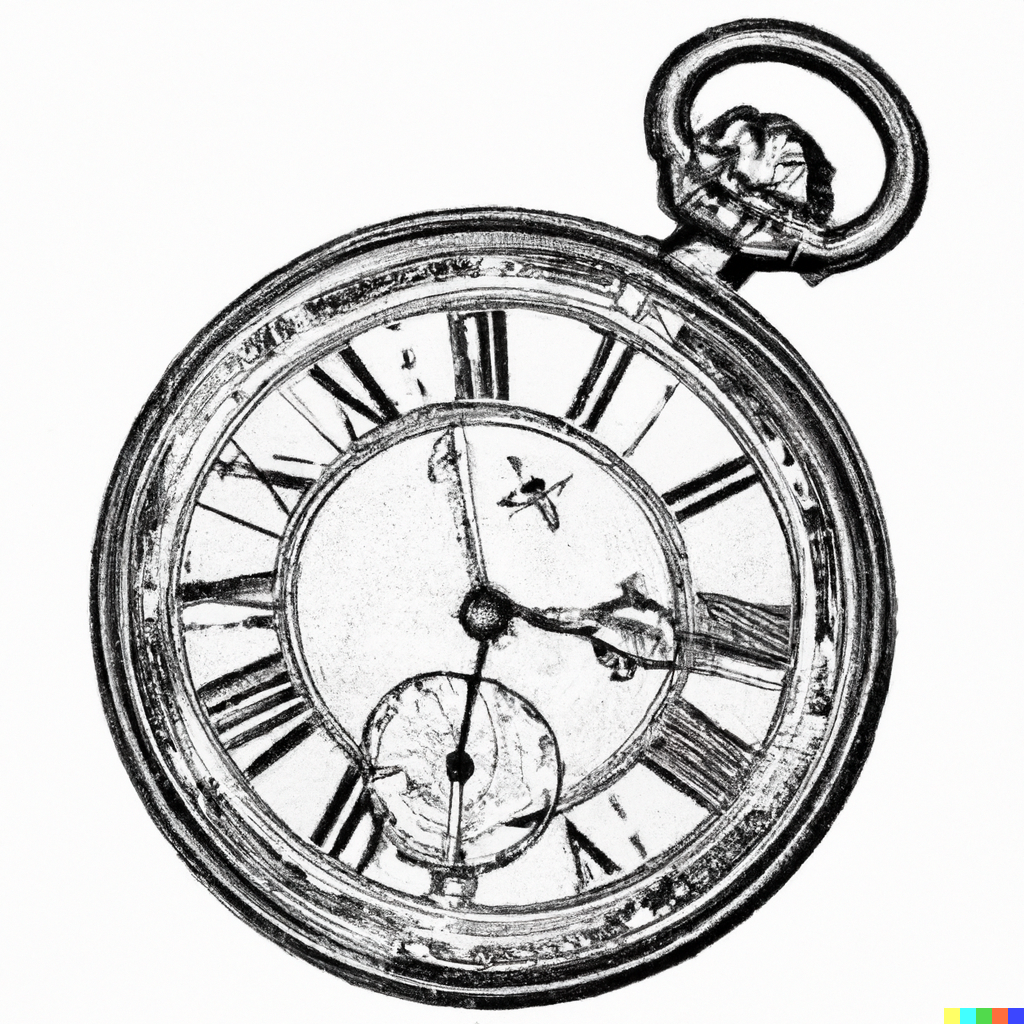
\includegraphics[width=3cm]{image/engraving-of-an-old-watch}
        \end{columns}
    \end{frame}

    \begin{frame}
        \transdissolve
        \frametitle{Liskov Principle}
        \framesubtitle{Exercice \execcounterdispinc{} de refactoring de 15 minutes}
        Refactoriser le code \url{https://github.com/St-Michel-IT/architecture-application/liskov-rectangle.py}.
        La fonction \lstinline{use_it} ne peut pas être utilisée avec la classe \lstinline{Square} sans modification.
        Refactoriser les classes \lstinline{Square} et \lstinline{Rectangle} pour qu'elles héritent d'une classe abstraite à développer et que \lstinline{use_it} fonctionne avec les deux classes.
        \bigbreak
        \begin{columns}
            \column{0.5\textwidth}
            Appliquer le TDD, rédiger les tests unitaires avant de coder.
            \bigbreak
            Commiter dans un dépôt Git, le schéma issu de l'exercice précédent, le code et les tests.
            \bigbreak
            Le travail de certains étudiants sera évalué.
            \column{0.5\textwidth}
            \centering
            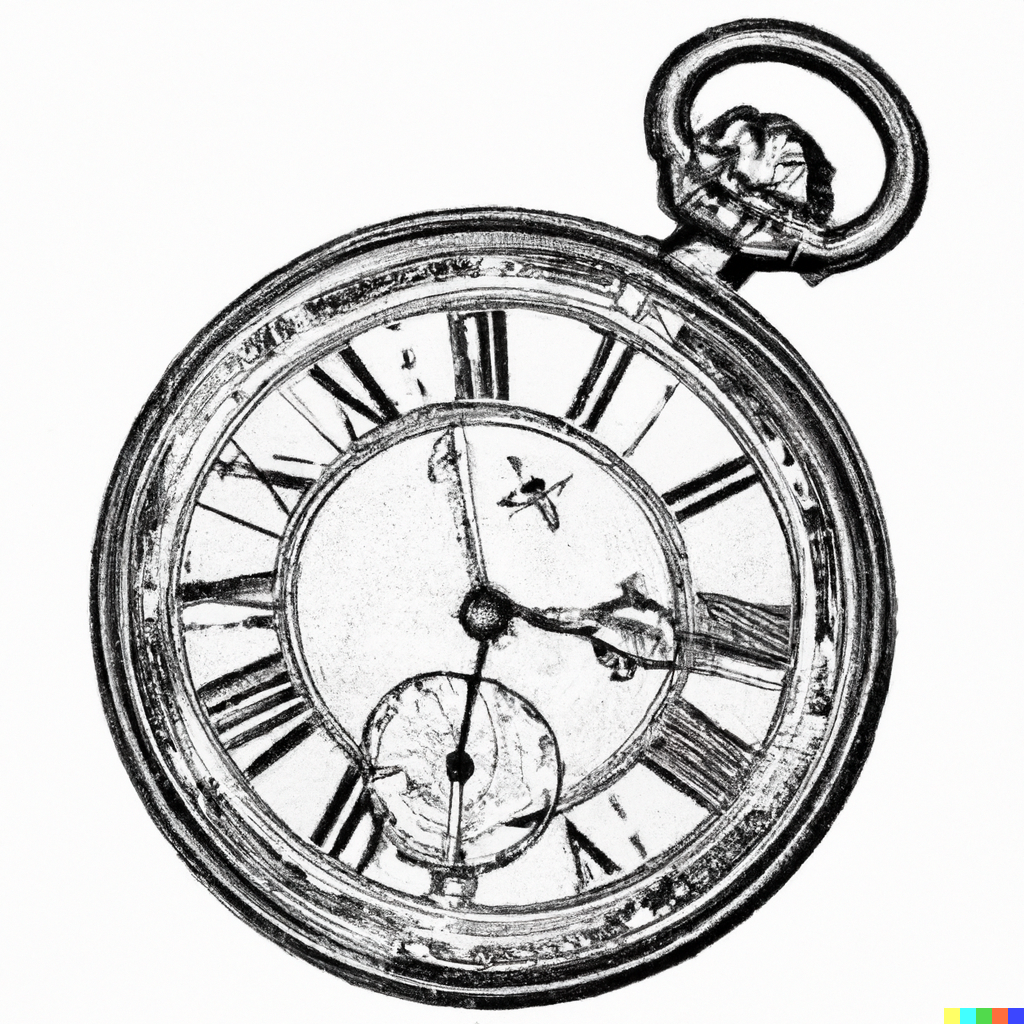
\includegraphics[width=3cm]{image/engraving-of-an-old-watch}
        \end{columns}
    \end{frame}

    \begin{frame}
        \transdissolve
        \frametitle{Interface Segragation Principle (ISP)}
        \framesubtitle{Définition\cref{cleanarchitecture}}
        Dépendre de quelque qui a un bagage que l'on utilise pas peut être une source de bugs inattendus.
        \bigbreak
        Pour éviter ce risque, il faut multiplier les interfaces plus petites pour mieux isoler l'impact d'une modification.
        \begin{columns}
            \column{0.5\textwidth}
            \centering
            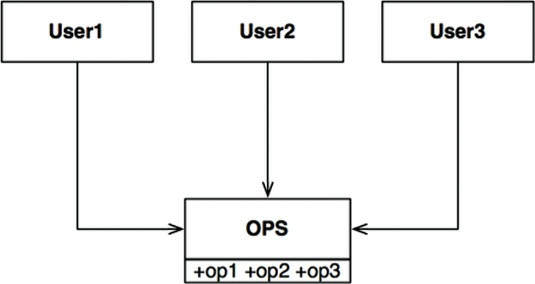
\includegraphics[width=5cm]{image/i-to-avoid} \\ A éviter \\
            \column{0.5\textwidth}
            \centering
            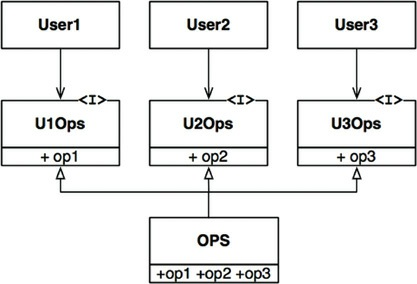
\includegraphics[width=5cm]{image/i-preferred} \\ A appliquer \\
        \end{columns}
    \end{frame}

    \begin{frame}
        \transdissolve
        \frametitle{Interface Segragation Principle}
        \framesubtitle{Définition\cref{cleanarchitecture}}
        \begin{columns}
            \column{0.5\textwidth}
            \centering
            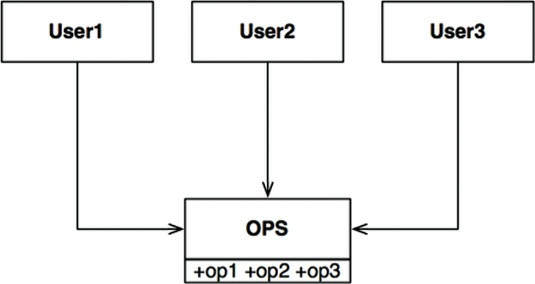
\includegraphics[width=5cm]{image/i-to-avoid} \\ A éviter \\
            \column{0.5\textwidth}
            \centering
            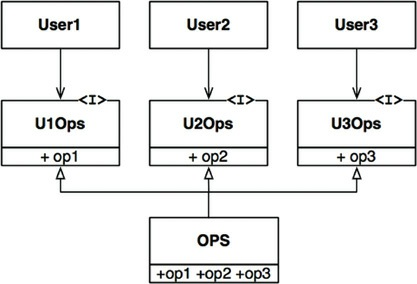
\includegraphics[width=5cm]{image/i-preferred} \\ A appliquer \\
        \end{columns}
        Dans le cas d'un langage typé statiquement, comme Java, à gauche on a une interface unique, et si il y a une modification dans une classe \lstinline{UserX}, recompilation, déploiement toutes les classes \lstinline{UserX} doivent être recompilées et redéployées même si elles ne sont pas modifiées.
        \bigbreak
        Ce problème n'existe pas avec l'approche à droite. \lstinline{Ops} peut être modifié sans avoir à recompiler les classes \lstinline{UserX}.
    \end{frame}

    \begin{frame}
        \transdissolve
        \frametitle{Interface Segregation Principle}
        \framesubtitle{Définition\cref{cleanarchitecture}}
        Question~:Pourquoi ce problème n'apparait pas avec les langages typés dynamiquement~?
        \pause
        \bigbreak
        Car le type est inféré au moment de l'exécution puisqu'il est dynamique.
        \begin{dangercolorbox}
            Cela ne veut pas dire qu'il ne faut pas respecter l'ISP dans ces langages.
            Les dépendances inutiles sont toujours à éviter, l'ISP est juste une raison de plus.
        \end{dangercolorbox}
        Quel rapport avec les dépendances aux packages distants (du web)~?
        \pause
        \bigbreak
        On ne connait pas le code de ces packages, on ne sait pas ce qu'ils contiennent.
        Le plus souvient, au mieux, on en connait les interfaces décrites dans la documentation.
    \end{frame}

    \begin{frame}
        \transdissolve
        \frametitle{Interface Segregation Principle}
        \framesubtitle{Exercice \execcounterdispinc{} de refactoring de 30 minutes}
        Dans le code \url{https://github.com/St-Michel-IT/architecture-application/blob/main/interface-segregation-payment.py}.
        \begin{itemize}
            \item Trouver les classes qui ne respectent pas l'ISP~.
            \item Refactoriser le code pour qu'il respecte l'ISP~. \textbf{Indice}~: Utiliser les classes abstraites.
        \end{itemize}
        \bigbreak
        \begin{columns}
            \column{0.5\textwidth}
            Commiter dans un dépôt Git, le schéma issu de l'exercice précédent, le code et les tests.
            \bigbreak
            Le travail de certains étudiants sera évalué.
            \column{0.5\textwidth}
            \centering
            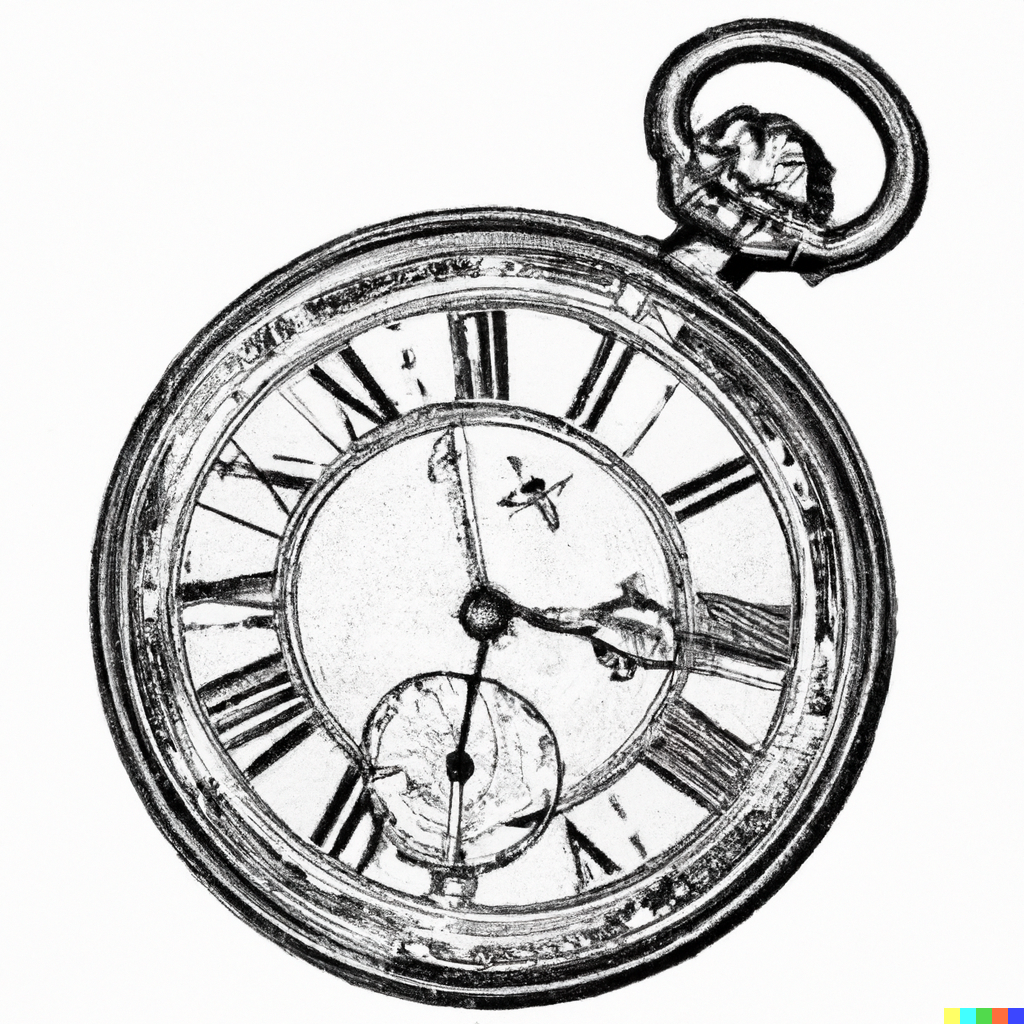
\includegraphics[width=3cm]{image/engraving-of-an-old-watch}
        \end{columns}
    \end{frame}

    \begin{frame}
        \transdissolve
        \frametitle{Dependency Inversion Principle (DIP)}
        \framesubtitle{Définition\cref{cleanarchitecture}}
        Dépendre des structures les plus stables, i.e., les moins volatiles.
        \bigbreak
        Tout changement dans une classe abstraite implique un changement dans les classes concrètes qui en héritent.
        L'inverse n'est pas vrai.
        Un changement dans une classe concrète n'implique pas forcément de modification dans les classes abstraites.
        \bigbreak
        Par conséquent les abstractions et les interfaces sont plus stables que les implémentations.
        \bigbreak
        Autrement dit, le DIP conseil, \textbf{tant que faire ce peut}, de dépendre des abstractions et non des implémentations.
        Les \lstinline{import}, \lstinline{use}, \lstinline{require}, \lstinline{include}, etc, doivent pointer vers des interfaces et non des classes concrètes.
        \begin{footnotesize}
            \begin{dangercolorbox}
                Il n'est pas réaliste de suivre de manière stricte cette règle.
                Tentez de l'appliquer quand c'est possible sans rajouter de complexité.
                Gardons en tête que certaines classes concrètes sont extrêmement stables comme \lstinline{String} de \lstinline{java.lang.string}.
            \end{dangercolorbox}
        \end{footnotesize}
    \end{frame}


    \begin{frame}
        \transdissolve
        \frametitle{Dependency Inversion Principle}
        \framesubtitle{Exercice \execcounterdispinc{} de refactoring de 15 minutes}
        Dans le code \url{https://github.com/St-Michel-IT/architecture-application/blob/main/dip-to-refactor.py}.
        \begin{itemize}
            \item il y a couplage entre la classe \lstinline{PowerSwitch} et \lstinline{LightBulb}.
            Alors qu'on peut être l'interrupteur d'autre chose qu'une ampoule.
            \item Refactoriser le code pour qu'il respecte l'DIP~. \textbf{Indice}~: Ajouter une classe abstraite.
            \item Ajouter une classe concrète \lstinline{Fan} qui implémente la nouvelle classe abstraite comme test.
        \end{itemize}
        \bigbreak
        \begin{columns}
            \column{0.6\textwidth}
            Appliquer le TDD, rédiger les tests unitaires avant de coder.
            \bigbreak
            Commiter dans un dépôt Git, le schéma issu de l'exercice précédent, le code et les tests.
            \bigbreak
            Le travail de certains étudiants sera évalué.
            \column{0.4\textwidth}
            \centering
            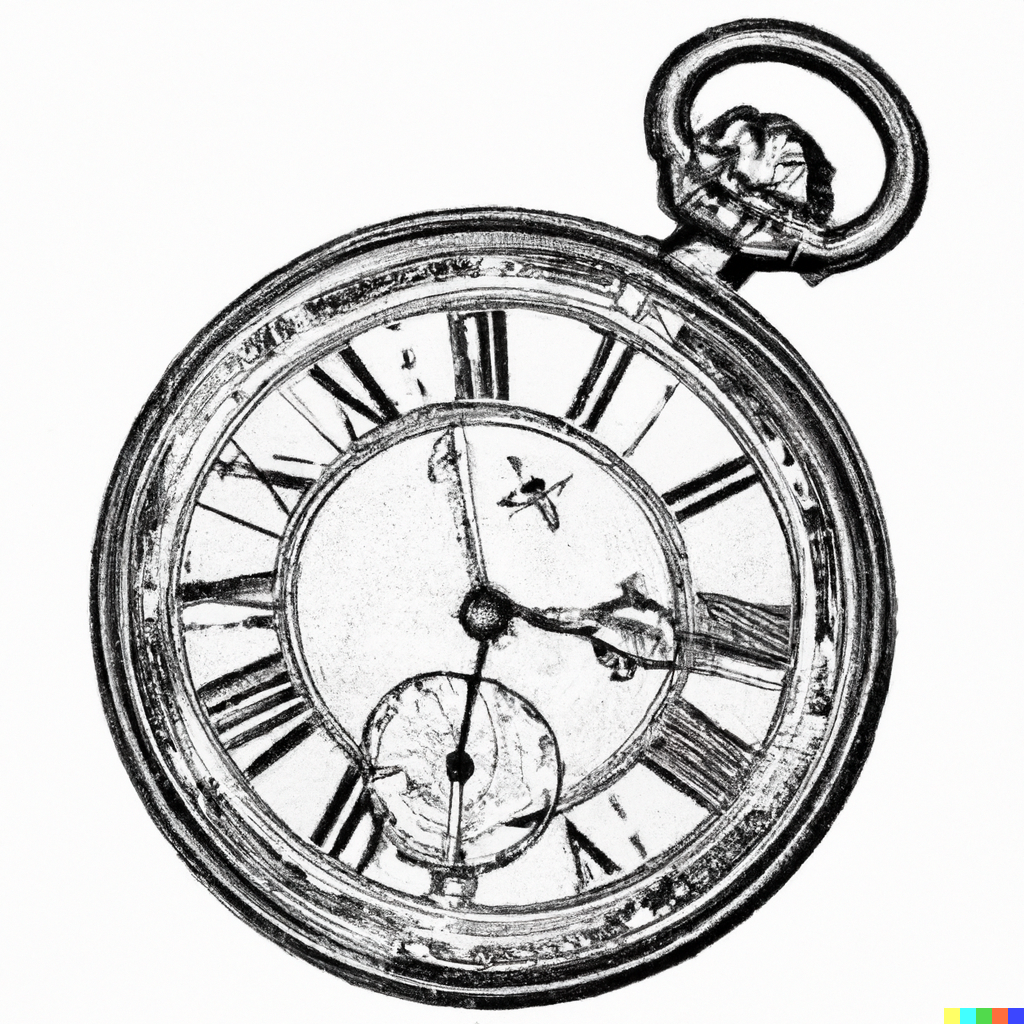
\includegraphics[width=3cm]{image/engraving-of-an-old-watch}
        \end{columns}
    \end{frame}

    \begin{frame}
        \transdissolve
        \frametitle{S.O.L.I.D.}
        \framesubtitle{Conclusion}
        S.O.L.I.D. est un ensemble de principes qui aident à solutionner des problèmes déjà vus aux chapitres précédents.
        \begin{itemize}
            \item Principalement les soucis de couplage trop fort \cref{sec:generalites}.
            \item Une des solutions récurrente pour respecter les principes S.O.L.I.D. est de créer des abstractions.
            Cela rappel à la mesure de l'\textquote{Abstractness} $A$ mesurée au précédent chapitre \cref{sec:les-mesures}.
        \end{itemize}
        \bigbreak
        \centering
        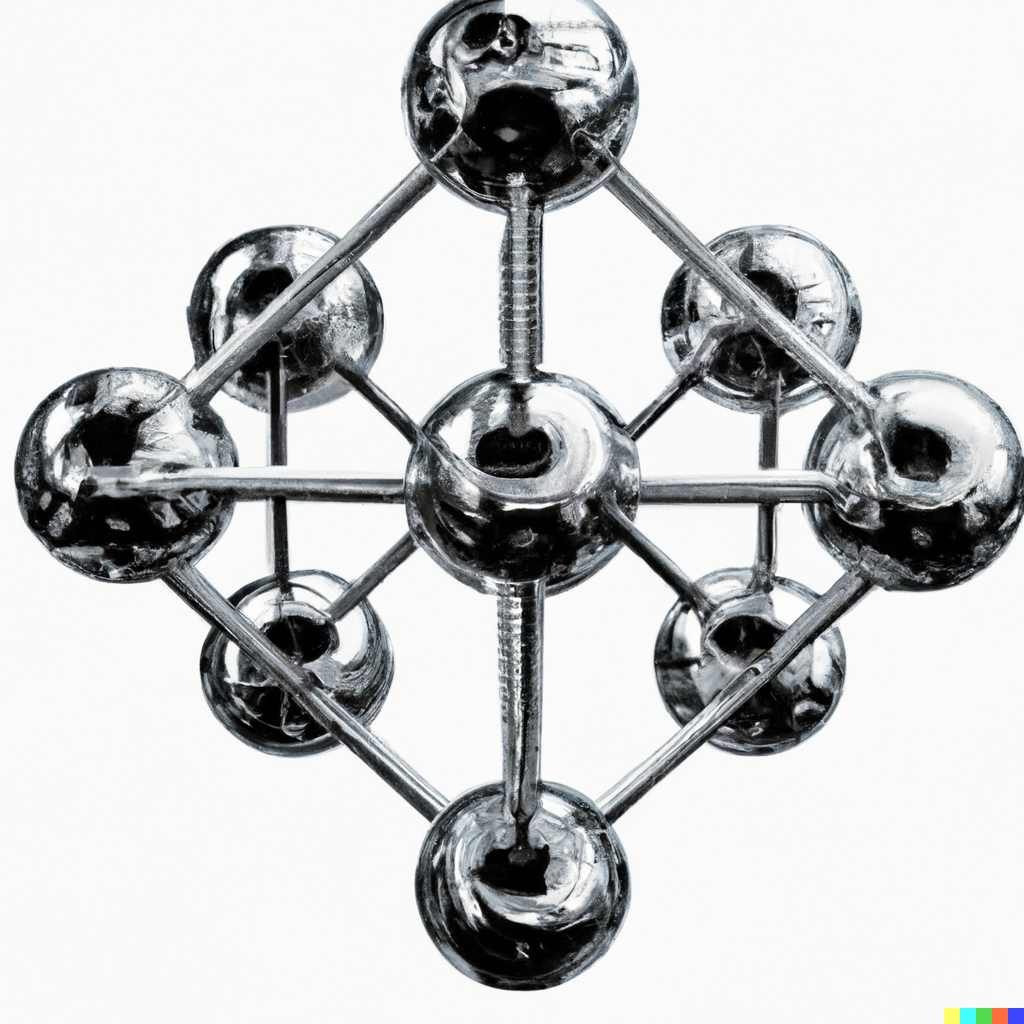
\includegraphics[width=4cm]{image/carbon-atoms}
    \end{frame}


    \section{High Level Desgin (HLD)}\label{sec:high-level-design}

    \begin{frame}
        \transdissolve
        \frametitle{High Level Desgin (HLD)}
        \framesubtitle{Déifiniton \footnote{Carnegie Mellon UNiverety, Philip Koopman, \url{https://course.ece.cmu.edu/~ece642/lectures/12_Architecture_HLD.pdf}}}
        Le HLD est une description de l'architecture, une vue d'ensemble d'un système qui peut être un produit entier.
        \bigbreak
        On peut entre autre utiliser plusieurs diagrammes pour décrire le HLD~:
        \begin{itemize}
            \item UML avec le diagramme de séquence.
            \item UML avec le diagramme d'activité.
            \item UML avec \textquote{Use case}.
            \item Diagramme \textquote{Data Flow}.
        \end{itemize}
        \bigbreak
        Le HLD est une vue d'ensemble, il ne rentre donc pas dans les détails.
        Ces derniers sont dans les diagrammes de la mid-level architecture.
    \end{frame}

    \begin{frame}
        \transdissolve
        \frametitle{High Level Desgin (HLD)}
        \framesubtitle{Exemples de diagrammes}
        \begin{columns}
            \column{0.5\textwidth}
            \centering
            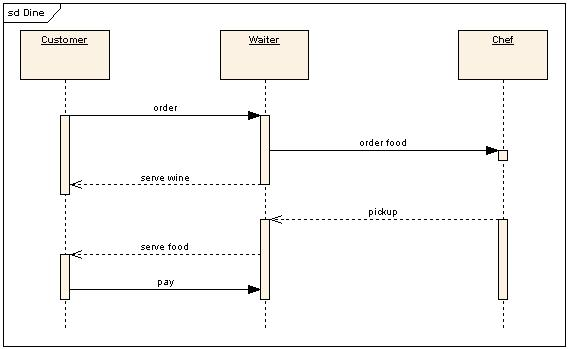
\includegraphics[width=3.5cm]{image/uml-sequence-diagram} \\ UML, diagramme de séquence \\
            \column{0.5\textwidth}
            \centering
            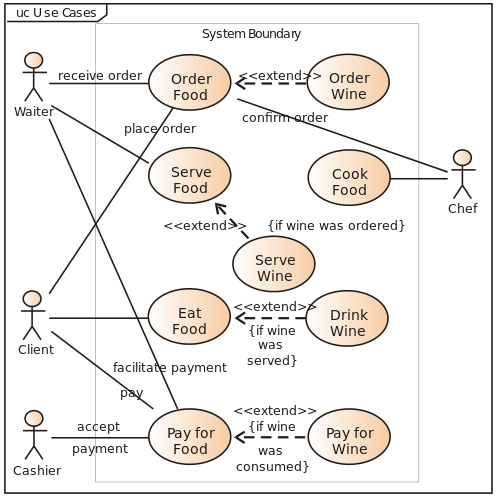
\includegraphics[width=3.5cm]{image/uml-use-case-diagram} \\ UML, diagramme \textquote{Use case} \\
        \end{columns}
        \begin{columns}
            \column{0.5\textwidth}
            \centering
            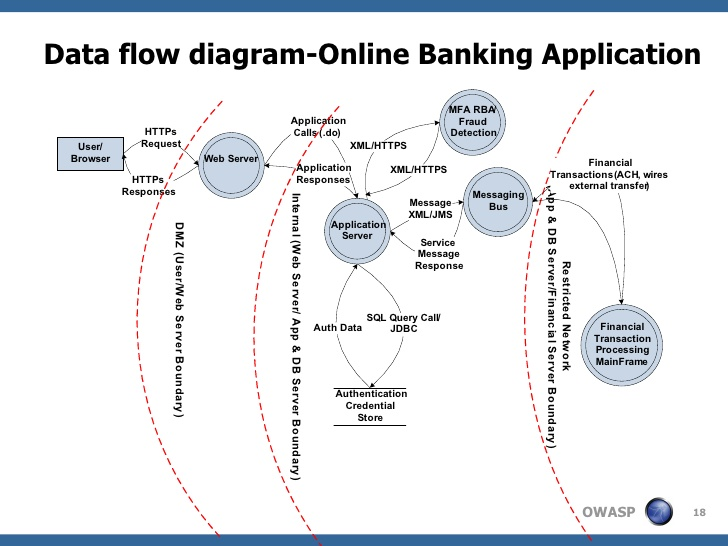
\includegraphics[width=4cm]{image/data-flow-diagramm-online-banking-application} \\ Diagramme Data Flow \\
            \column{0.5\textwidth}
            \centering
            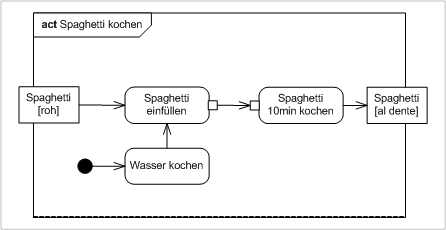
\includegraphics[width=4cm]{image/uml-activity-diagram} \\ UML, diagramme d'activité \\
        \end{columns}
    \end{frame}

    \begin{frame}
        \transdissolve
        \frametitle{High Level Desgin (HLD)}
        \framesubtitle{Bonnes pratiques}
        \begin{itemize}
            \item C'est un ou plusieurs diagrammes
            \item S'applique à tous les composants du système, soft, hard, réseau, etc.
            \item S'applique à toutes les interfaces entre ces composants.
            \item Évolue avec les spécifications.
            \item Ne comprends pas trop de détails qui compliquent la compréhension.
            D'autres diagrammes sont là pour ça.
            \item Utiliser des outils dédiés, comme Draw.io ou PlantUML pour les diagrammes UML~.
        \end{itemize}
    \end{frame}


    \section{Service-Oriented Architecture}\label{sec:soa}

    \begin{frame}
        \transdissolve
        \frametitle{Architectures Orientées Service}
        \framesubtitle{Définition\cref{fundsofsoftarch}}
        \textquote{Service-Oriented Architecture} (SOA) en anglais, est un style d'architecture logicielle qui vise à concevoir des applications comme un ensemble de services.
        \bigbreak
        Vu de l'extérieur, un service expose une interface qui permet d'interagir avec lui.
        Il y a de plusieurs services, chacun dédié à une tâche spécifique.
        Ils communiquent tous avec la même base de données.
        \begin{columns}
            \column{0.5\textwidth}
            Cette une approche considérée comme l'opposé de l'approche \textquote{monolithique}.

            Le client peut-être un navigateur web, une application mobile, un autre service, etc.
            \column{0.5\textwidth}
            \centering
            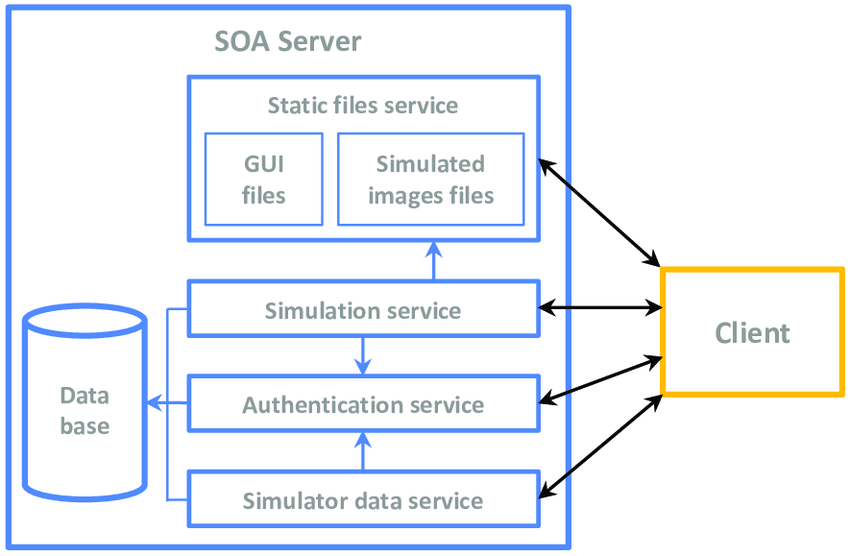
\includegraphics[width=5cm]{image/soa-server}
        \end{columns}
    \end{frame}

    \begin{frame}
        \transdissolve
        \frametitle{Architectures Orientées Service}
        \framesubtitle{Définition\cref{fundsofsoftarch}}
        Cette approche est hybride entre le monolithique et les microservices.
        \bigbreak
        Elle est considérée comme plus souple que le monolithique et plus simple que le microservices.
        \bigbreak
        La meilleurs flexibilité vient entre autre du fait que les services peuvent être développés dans des technologies différentes.
        Ils peuvent être déployés indépendamment.
        \bigbreak
        \begin{columns}
            \column{0.5\textwidth}
            Un \textquote{Reverse Proxy} peut-être utilisé pour rediriger les requêtes vers le bon service tout en donnant l'impression de n'avoir qu'un seul serveur.
            \column{0.5\textwidth}
            \centering
            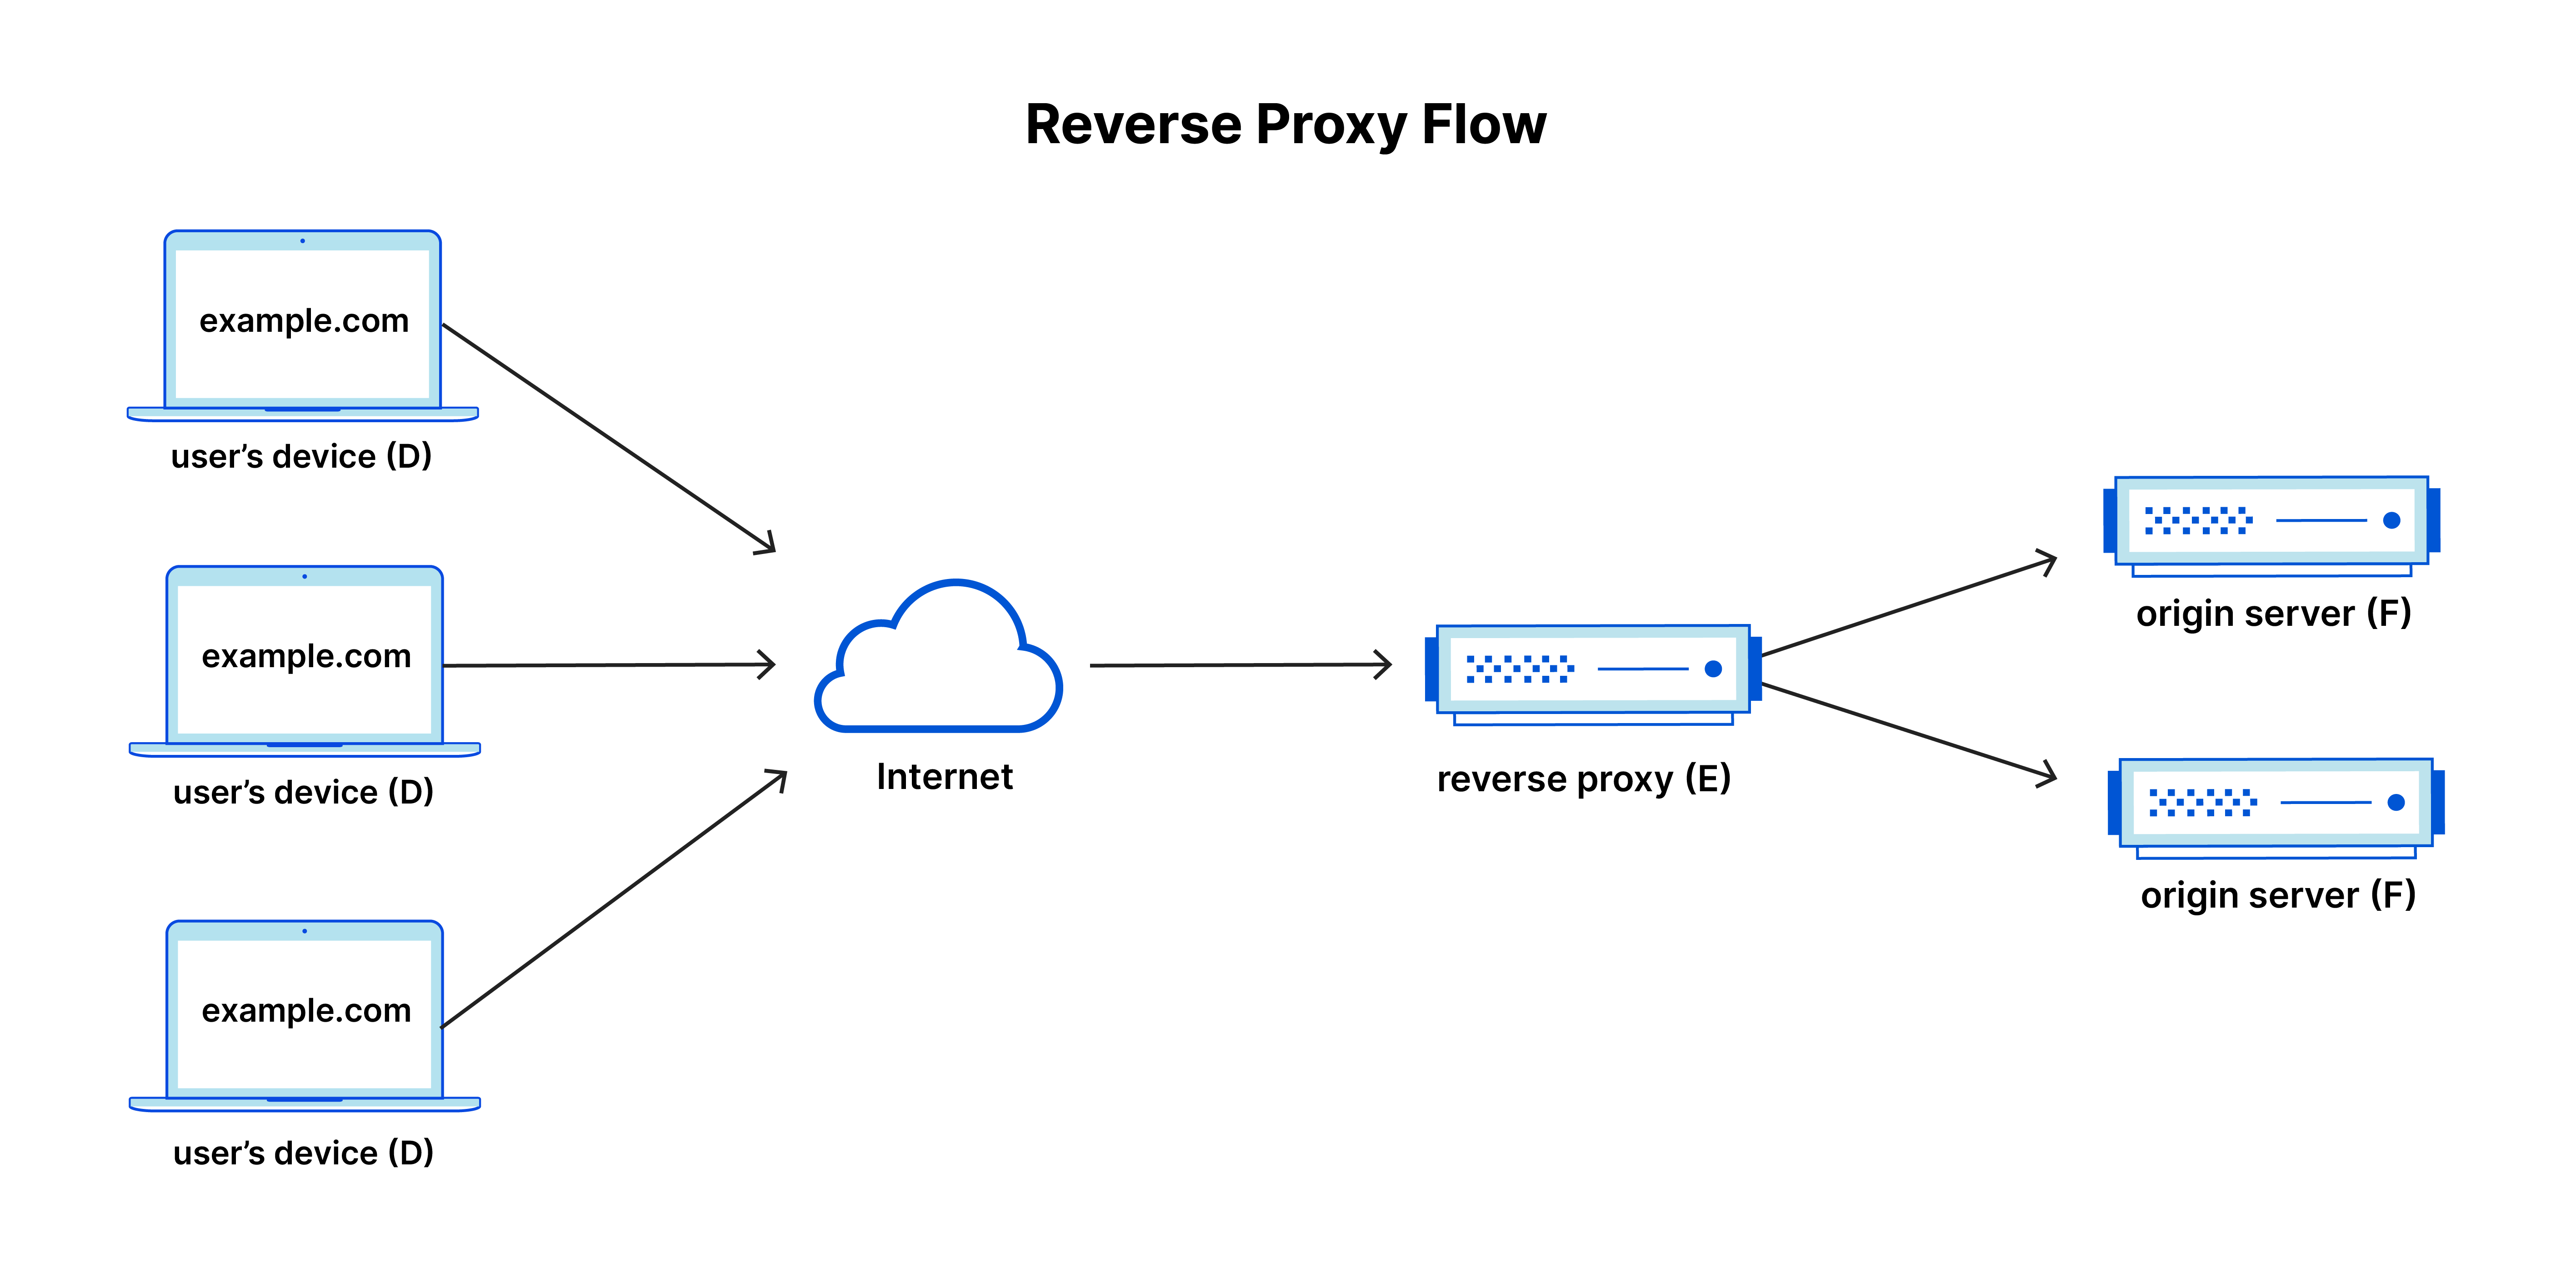
\includegraphics[width=6cm]{image/reverse-proxy-flow}
        \end{columns}
    \end{frame}

    \begin{frame}
        \transdissolve
        \frametitle{Architectures Orientées Service}
        \framesubtitle{Définition\cref{fundsofsoftarch}}
        Quel est l'intérêt d'avoir une ou des bases de données communes à tous les services~?
        \pause
        \bigbreak
        \begin{itemize}
            \item Éviter la redondance de données.
            \item Éviter les incohérences de données.
            \item Éviter les problèmes de synchronisation.
            \item Éviter les problèmes de sécurité.
            \item Éviter un impact sur les performances lié à la duplication et à la com'.
        \end{itemize}
        \begin{dangercolorbox}
            SOA n'est pas un standard ou un protocole, c'est un style d'architecture.
        \end{dangercolorbox}
    \end{frame}

    \begin{frame}
        \transdissolve
        \frametitle{Introduction aux Architectures Orientées Services}
        \framesubtitle{Introduction aux Architectures Orientées Services\footnote{\label{newop-soa}A Guide to Service-Oriented Architecture (SOA) Styles, \url{https://www.newnop.com/blog/a-guide-to-service-oriented-architecture-(soa)-styles}}}
        \begin{columns}
            \column{0.5\textwidth}
            Plusieurs variantes de SOA ont vues le jour~:
            \column{0.5\textwidth}
            \centering
            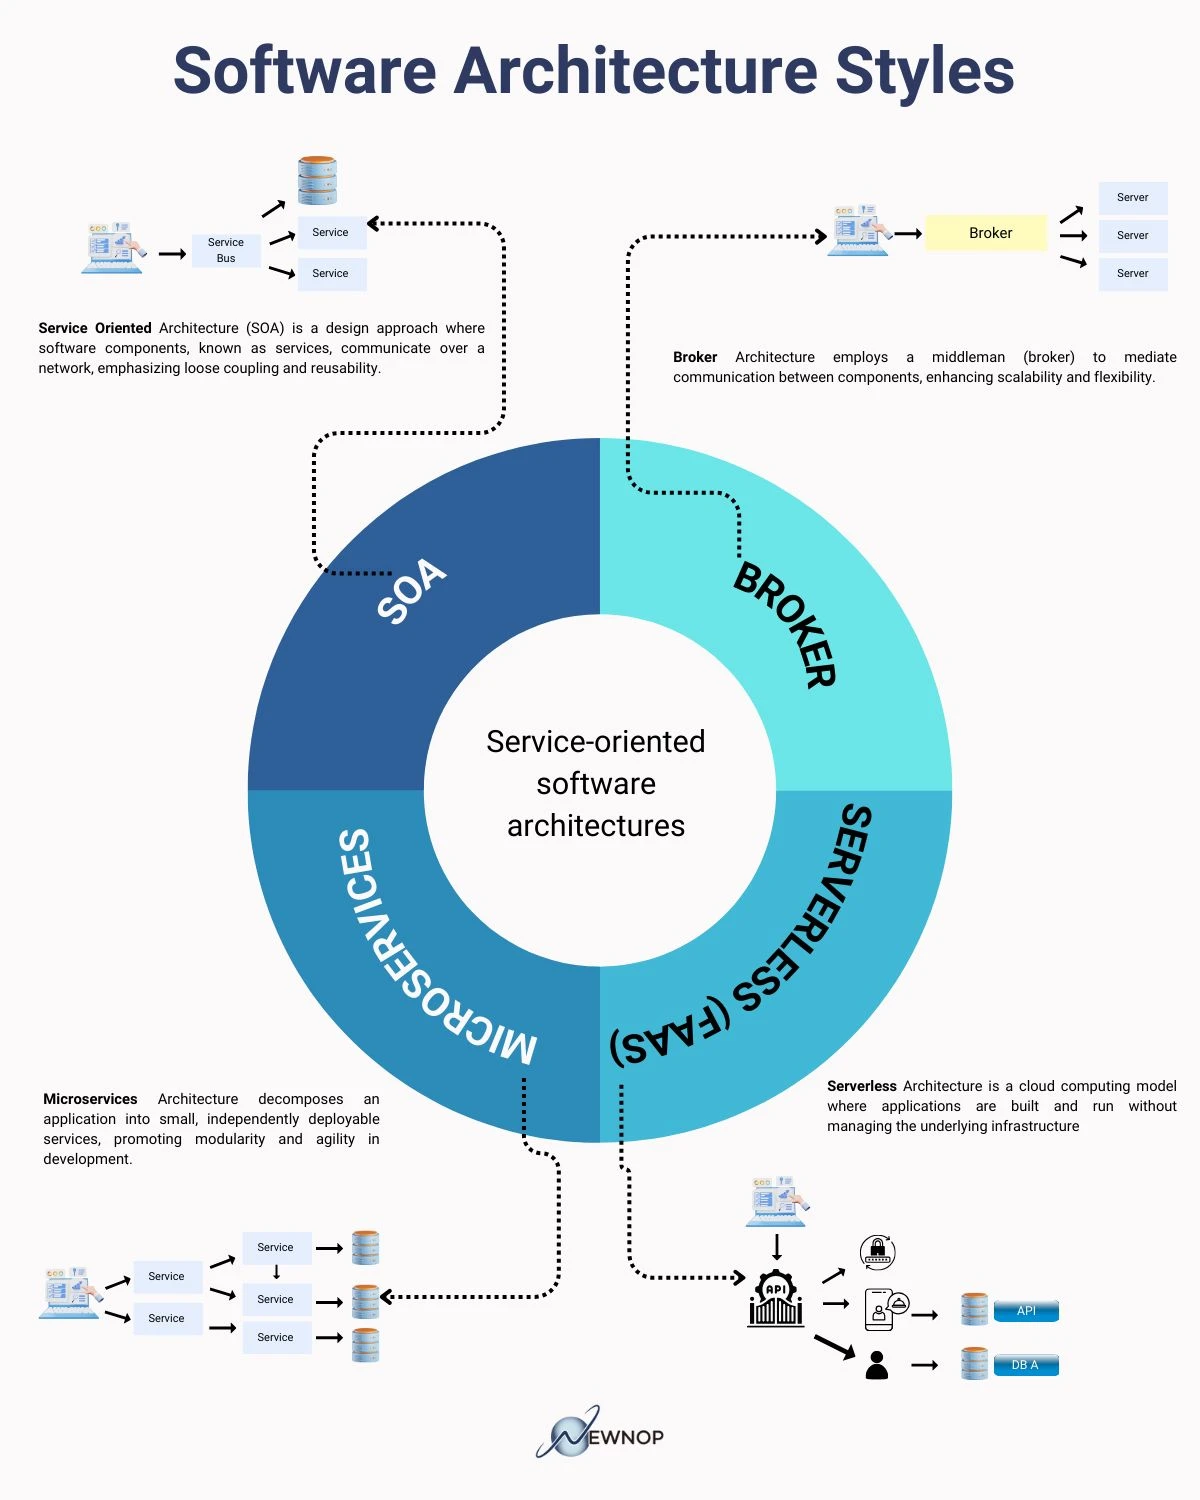
\includegraphics[width=5cm]{image/diversity-of-soa}
        \end{columns}
    \end{frame}

    \begin{frame}
        \transdissolve
        \frametitle{Introduction aux Architectures Orientées Services}
        \framesubtitle{Introduction aux Architectures Orientées Services\cref{newop-soa}}
        \begin{footnotesize}
            \begin{itemize}
                \item \textbf{broker}~: En s'appuyant sur les fondations de l'architecture orientée services (SOA), le style Broker introduit une entité centrale appelée \textquote{broker} pour gérer la communication entre différents services.
                Imaginez ce \textquote{broker} comme un contrôleur de trafic expérimenté, routant habilement les messages et assurant un flux de communication fluide.
                \item \textbf{Microservice}~: En poussant le concept de modularité à un niveau supérieur, l'architecture des microservices est devenue un choix populaire pour la construction d'applications logicielles modernes.
                Ce style préconise de décomposer les applications en services encore plus petits, indépendants et autonomes.
                Pensez à ces services comme à des microcosmes individuels au sein de l'écosystème applicatif plus large, chacun accomplissant une tâche spécifique.
                \item \textbf{Serverless}~: le style architectural \textquote{serverless}, une approche native du cloud qui redéfinit la manière dont les applications sont construites et déployées.
                Au lieu de provisionner et de gérer des serveurs, les développeurs écrivent des fragments de code appelés « fonctions » qui sont déclenchés par des événements spécifiques.
                La gestion d'un maximum de l'infrastructure est laissée à une équipe dédiée - c'est l'essence du \textquote{serverless}.
                Quel(s) produit(s) cloud \textquote{serverless} réputé connaissez-vous~?
            \end{itemize}
            Quels sont les avantages et inconvenient de ces styles~?
        \end{footnotesize}
    \end{frame}


    \section{Les architectures des échanges du web}\label{sec:web-com}

    \subsection{Communication client-serveur}\label{subsec:web-com-server-client}

    \begin{frame}
        \transdissolve
        \frametitle{Les architectures Client-Serveur}
        \framesubtitle{Les protocoles entre navigateur et serveur}
        Si le client est un navigateur web, les protocoles seront le HTTP et les protocoles construits au dessus.
        \bigbreak
        \centering
        
\includegraphics[width=10cm]{image/browser-soa-protocols.drawio}
        \flushleft
        Que peut-on échanger au dessus de HTTP entre le navigateur et le serveur~?
        \pause
        \bigbreak
        Des données brutes aux formats JSON, XML, HTML, etc.

        Potentiellement dans un autre protocole comme JSON-RPC, OpenID Connect, SOAP over HTTP, REST, etc.
    \end{frame}

    \begin{frame}
        \transdissolve
        \frametitle{Les architectures Client-Serveur}
        \framesubtitle{Les protocoles entre serveurs}
        Si le client est une autre machine, beaucoup plus de protocoles sont disponibles.
        \bigbreak
        \centering
        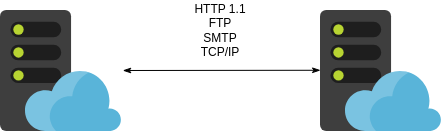
\includegraphics[width=10cm]{image/m2m-soa-protocols.drawio}
        \flushleft
        Que peut-on échanger au dessus de HTTP entre serveurs~?
        \pause
        \bigbreak
        Des données brutes aux formats JSON, XML, etc.

        Potentiellement dans un autre protocole comme SOAP over SMTP, SOAP over FTP, SOAP over HTTP, etc.
    \end{frame}

    \subsection{Appel de procédure}\label{subsec:rpc}

    \begin{frame}
        \transdissolve
        \frametitle{Appel de procédure}
        \framesubtitle{Définition}
        Couramment appelé RPC pour \textquote{Remote Procedure Call} en anglais.
        \bigbreak
        Ensemble de protocoles qui permettent à un programme client de demander à un serveur d'exécuter une fonction/procédure/programme.
        Le retour de cette procédure, i.e., la réponse est renvoyée au client.
        \bigbreak
        Les premières standardisations dans une RFC datent de 1976.
        \bigbreak
        C'est globalement une communication inter-process.
        \bigbreak
        Ces appels à des méthodes et les réponses en retour sont souvent sérialisés en JSON ou XML~.
        Ces données sérialisées sont ensuite envoyées en HTTP, le plus souvent.
        \bigbreak
        Fort de leur standardisation, on trouve leur implémentation côté et serveur dans tous les langages de programmation courants.
    \end{frame}

    \begin{frame}[fragile]
        \transdissolve
        \frametitle{Appel de procédure}
        \framesubtitle{1998 le XML-RPC\footnote{Simple cross-platform distributed computing, based on the standards of the Internet., \url{http://1998.xmlrpc.com/}}}
        Cette appel de procédure distant utilise le HTTP pour le transport et le XML pour la sérialisation.

        Exemple d'appel~:
        \begin{lstlisting}[language=xml,basicstyle=\ttfamily\tiny]
<?xml version="1.0"?>
    <methodCall>
        <methodName>Teststatut</methodName>
        <params>
        <param>
            <value><i4>10</i4></value>
        </param>
        </params>
    </methodCall>
        \end{lstlisting}
        Exemple de réponse~:
        \begin{lstlisting}[language=xml,basicstyle=\ttfamily\tiny]
<?xml version="1.0"?>
    <methodResponse>
        <params>
        <param>
            <value><string>Statut : OK</string></value>
        </param>
        </params>
    </methodResponse>
        \end{lstlisting}
    \end{frame}

    \begin{frame}
        \transdissolve
        \frametitle{Appel de procédure}
        \framesubtitle{1998, le XML-RPC}
        Quel est l'avantage du XML-RPC~?
        \pause
        \bigbreak
        Les XML ont une grammaire vérifiable grâce à un schéma XSD~.
        Le JSON de base n'a pas de grammaire.
        Il faut définir un schéma JSON avec CDDL\footnote{Concise Data Definition Language (CDDL): A Notational Convention to Express Concise Binary Object Representation (CBOR) and JSON Data Structures., \url{https://datatracker.ietf.org/doc/html/rfc8610}} par exemple.

        Quel est l'inconvénient du XML par rapport au JSON~?
        \pause
        \bigbreak
        Le XML est plus verbeux que le JSON, donc plus difficile à lire et plus long à transférer.
        \bigbreak
        \textquote{Rappel}~: On peut parser du XML en JS dans le navigateur \url{https://developer.mozilla.org/en-US/docs/Web/XML/Parsing_and_serializing_XML}
    \end{frame}

    \begin{frame}[fragile]
        \transdissolve
        \frametitle{Appel de procédure}
        \framesubtitle{Le JSON-RPC 1 et 2\footnote{JSON-RPC, A light weight remote procedure call protocol. It is designed to be simple!, \url{https://www.jsonrpc.org/}}}
        Le JSON se popularise au milieu des années 2000 mais est standardisé seulement en 2013\footnote{The JavaScript Object Notation (JSON) Data Interchange Format, \url{https://www.rfc-editor.org/rfc/rfc7158}}.

        La dernière version de JSON-RPC, la 2.0, celle à utiliser, date de 2013 également.

        Exemple d'appels et réponses~:
        \begin{lstlisting}[language=java,basicstyle=\ttfamily\tiny]
// Avec des "named parameters"
{"jsonrpc": "2.0", "method": "subtract", "params": {"subtrahend": 23, "minuend": 42}, "id": 3} // Appel -->
{"jsonrpc": "2.0", "result": 19, "id": 3} // Réponse <--
// Équivalent aux "positional parameters"
{"jsonrpc": "2.0", "method": "subtract", "params": [42, 23], "id": 1} // Appel -->
{"jsonrpc": "2.0", "result": 19, "id": 1} // Réponse <--
// Une notification n'a pas de "id" et donc pas ed réponse
{"jsonrpc": "2.0", "method": "update", "params": [1,2,3,4,5]} // Appel -->
{"jsonrpc": "2.0", "method": "foobar"} // Appel -->
// Batch de commandes, les mêmes commandes sont dans un tableau, possible pour les notifications également
[{"jsonrpc": "2.0", "method": "sum", "params": [1,2,4], "id": "1"},
    {"jsonrpc": "2.0", "result": 19, "id": "2"}] // Appel -->
[{"jsonrpc": "2.0", "result": 7, "id": "1"},
    {"jsonrpc": "2.0", "result": 19, "id": "2"}] // Réponse <--
        \end{lstlisting}
    \end{frame}

    \begin{frame}
        \transdissolve
        \frametitle{Appel de procédure}
        \framesubtitle{JSON-RPC}
        Quel sont les avantages du JSON-RPC~?
        \pause
        \bigbreak
        \begin{itemize}
            \item Le JSON est plus léger que le XML, donc plus vite transféré.
            \item Le JSON est plus facilement lisible que le XML~.
            \item Facile à implémenter en JS dans le navigateur ou à utiliser avec une librairie.
        \end{itemize}
        \bigbreak
        Quel est l'inconvénient du JSON par rapport au XML~?
        \pause
        \bigbreak
        Pas de schéma du JSON de la charge utile!
        \bigbreak
        Voir l'exemple de serveur qui \href{https://github.com/St-Michel-IT/testing/blob/master/ble_to_rpc.py}{expose le BLE sur le HTTP over JSON-RPC}~.
    \end{frame}

    \begin{frame}[fragile]
        \transdissolve
        \frametitle{Appel de procédure}
        \framesubtitle{gRPC\footnote{gRPC, A high performance, open source universal RPC framework, \url{https://grpc.io/}}}
        gRPC est un RPC open source développé par Google qui l'a libéré en 2015.
        \bigbreak
        Il est basé sur le protocole HTTP/2 et utilise le format de sérialisation de données Protobuf A.K.A Protocol Buffer.
        Protobuff est un format binaire défini par un schéma.
        \bigbreak
        Pourquoi un format binaire~?
        % listing
        \begin{lstlisting}
>>> from sys import getsizeof # La taille en octets d'un objet
>>> from struct import pack " Struct pour parser ou générer du binaire
>>> print("Compare with string")
>>> struct_object = pack(">H", 0xffff) # H == uInt16, unsigned short
>>> print(0xffff)
>>> print("lentgh of the string:", getsizeof("65535"))
>>> print("lentgh of the struct:", getsizeof(struct_object))
Compare with string
65535
lentgh of the string: 54
lentgh of the struct: 35
        \end{lstlisting}
    \end{frame}

    \begin{frame}
        \transdissolve
        \frametitle{Appel de procédure}
        \framesubtitle{Pourquoi Protobuff dans le RPC}
        Un schéma réduit les bugs possibles.
        \begin{itemize}
            \item Comme par exemple un format de donnée incohérent, une balise ou une clé en JSON qui ne respecte pas la hiérarchie attendue.
            \item Type de donnée incohérent
            \item Valeur incohérente, comme 6000000 dans un champ qui attend un entier 16 bits.
            \item Sûrement d'autres\ldots
        \end{itemize}
        \bigbreak
        Toutes les erreurs ci-dessus vont induire un crash lors de la sérialisation des données.
        Les données erronées ne peuvent donc pas être envoyées au client ou au serveur.
        D'où la diminution des bugs possibles.
    \end{frame}

    \begin{frame}
        \transdissolve
        \frametitle{Appel de procédure}
        \framesubtitle{Pourquoi Protobuff dans le RPC}
        Rappel sur la sérialisation des données, les grandes familles~:
        \bigbreak
        \centering
        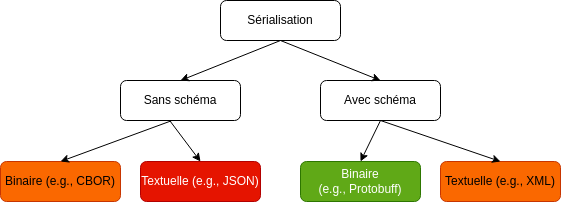
\includegraphics[width=10cm]{image/serialization.drawio} \\ Échelle des problèmes potentiels du vert au rouge \\
    \end{frame}

    \begin{frame}
        \transdissolve
        \frametitle{Appel de procédure}
        \framesubtitle{gRPC}
        Quel sont les avantages du gRPC~?
        \pause
        \bigbreak
        \begin{itemize}
            \item Un schéma de données qui réduit les bugs possibles.
            \item Le HTTP/2 est plus rapide que le HTTP/1.1.
            \item Le format binaire est plus léger que le JSON~.
        \end{itemize}
        \bigbreak
        Quel sont les inconvénients du gRPC~?
        \pause
        \bigbreak
        \begin{itemize}
            \item Il y a des étapes supplémentaires d'encodage et de décodage des données.
            \item Plus difficile à utiliser sans librairie et intégrer dans le navigateur.
            \item Impossible de lire la charge utile sans décoder.
        \end{itemize}
    \end{frame}

    \begin{frame}
        \transdissolve
        \frametitle{Appel de procédure}
        \framesubtitle{Conclusion}
        Les 3 types d'appels de procédure vus sont très standardisés.
        Les librairies pour les implémenter sont disponibles dans tous les langages de programmation courants.
        Souvent depuis des années et donc robustes.
        \bigbreak
        On peut les intégrer dans de nombreux systèmes, serveurs, navigateurs, applications mobiles, etc.
        \bigbreak
        L'\lstinline{id} dans la requête et la réponse permet d'envoyer un batch de requêtes et d'y associer les réponses.
        \bigbreak
        Ils sont reconnus pour leur simplicité d'utilisation, c'est presque aussi simple d'appeler une méthode sur une machine distante qu'en local.
        Vu comme cela on comprends par contre qu'il y a un très fort couplage entre le client et le serveur.
        Et donc un manque de flexibilité.
    \end{frame}

    \subsection{API REST}\label{subsec:api-rest}


    \begin{frame}
        \transdissolve
        \frametitle{API REST}
        \framesubtitle{Définition\footnote{Une API REST, qu'est-ce que c'est~?, \url{https://www.redhat.com/fr/topics/api/what-is-a-rest-api}}}
        \begin{footnotesize}
            Les API REST aussi parfois appelées API RESTful sont des API qui respectent les contraintes de l'architecture REST (Representational State Transfer) de Roy Fielding.
            \bigbreak
            Ces contraintes sont~:
            \begin{itemize}
                \item Client-serveur~: Le client et le serveur sont séparés.
                \item Stateless~: Chaque requête du client doit contenir toutes les informations nécessaires pour être traitée par le serveur.
                \item Cacheable~: Les réponses doivent être explicitement ou implicitement marquées comme cacheable ou non.
                \item Layered system~: Le client ne doit pas savoir si il communique avec le serveur ou un intermédiaire.
                \item Code on demand (optional)~: Le serveur peut envoyer du code au client pour être exécuté.
                \item Une interface uniforme entre les composants qui permet un transfert standardisé des informations~: Les ressources sont identifiées par des URI, les opérations sont standardisées (GET, POST, PUT, DELETE, etc), les réponses sont auto-descriptives.
            \end{itemize}
        \end{footnotesize}
    \end{frame}

    \begin{frame}[fragile]
        \transdissolve
        \frametitle{API}
        \framesubtitle{Définition}
        Aucune contrainte donc sur le langage de programmation, le système d'exploitation, le type de donnée, etc.
        \bigbreak
        De nombreuses libraries existent pour implémenter des API REST dans tous les langages de programmation courants.
        \bigbreak
        Par exemple dans un serveur Flask avec \href{https://flask-restful.readthedocs.io/en/latest/}{Flask-RESTful}~:
        \begin{lstlisting}[language=python,basicstyle=\ttfamily\tiny]
from flask import Flask
from flask_restful import Resource, Api

app = Flask(__name__)
api = Api(app)


class Hello(Resource):
    def get(self):
        return {'hello': 'world'}


api.add_resource(Hello, '/hello')

if __name__ == '__main__':
    app.run(debug=True)
        \end{lstlisting}
    \end{frame}

    \begin{frame}[fragile]
        \transdissolve
        \frametitle{API}
        Quelques exemples d'API REST avec des POST et aussi des arguments grâce à la librairie \lstinline{webargs} sur leur \href{https://github.com/marshmallow-code/webargs/blob/dev/examples/flaskrestful_example.py}{GitHub}.
        % Python listing
        \begin{lstlisting}[language=python,basicstyle=\ttfamily\tiny]
class DateAddResource(Resource):
    dateadd_args = {
        "value": fields.Date(required=False),
        "addend": fields.Int(required=True, validate=validate.Range(min=1)),
        "unit": fields.Str(
            load_default="days", validate=validate.OneOf(["minutes", "days"])
        ),
    }

    @use_kwargs(dateadd_args)
    def post(self, value, addend, unit):
        """A date adder endpoint."""
        value = value or dt.datetime.utcnow()
        if unit == "minutes":
            delta = dt.timedelta(minutes=addend)
        else:
            delta = dt.timedelta(days=addend)
        result = value + delta
        return {"result": result.isoformat()}


# This error handler is necessary for usage with Flask-RESTful
@parser.error_handler
def handle_request_parsing_error(err, req, schema, *, error_status_code, error_headers):
    """webargs error handler that uses Flask-RESTful's abort function to return
    a JSON error response to the client.
    """
    abort(error_status_code, errors=err.messages)
        \end{lstlisting}
    \end{frame}

    \subsection{La standardisation du contenu JSON}\label{subsec:api-json}

    \begin{frame}[fragile]
        \transdissolve
        \frametitle{Swagger}
        \framesubtitle{La spécification OpenAPI et le format Swagger}
        La spécification OpenAPI est une spécification pour décrire des API JSON~.
        Donc les API RESTful entre autre.
        \bigbreak
        Cette définition au format JSON ou YAML, dans un fichier appelé \textquote{Swagger}.
        \bigbreak
        Grâce à ce fichier de définition et des outils open source comme \lstinline{swagger-codegen}, on peut générer en local ou dans le CI~:
        \begin{itemize}
            \item La documentation de l'API~.
            \item Les clients pour les langages de programmation courants.
            \item Les serveurs pour les langages de programmation courants.
            \item Les tests.
            \item Une web UI pour tester l'API~.
            \item Many more\ldots
        \end{itemize}
    \end{frame}

    \begin{frame}[fragile]
        \transdissolve
        \frametitle{Swagger}
        \framesubtitle{La spécification OpenAPI et le format Swagger}
        Pour écrire le \textquote{Swagger} directement dans le code, il existe des librairies comme \lstinline{flasgger} qui permettent de générer la documentation de l'API à partir des docstrings des méthodes.

        Voir par exemple \url{https://github.com/flasgger/flasgger}.
        \begin{dangercolorbox}
            On remarque qu'on ne peut intégrer les deux libraries \lstinline{Flask-RESTful} et \lstinline{flasgger} ensemble dans un même serveur Flask.
            Il faut écrire la définition dans un fichier \textquote{Swagger} à part, \textquote{à l'ancienne}.

            La standardisation c'est propre mais c'est compliqué\ldots
        \end{dangercolorbox}
    \end{frame}

    \begin{frame}[fragile]
        \transdissolve
        \frametitle{JSON-LD}
        \framesubtitle{JSON Linked-Data\footnote{JSON for Linking Data, \url{https://json-ld.org/}}}
        Inspiré du web sémantique et de la sémantique des données, le JSON-LD est un format de données structurées qui permet de lier des données entre elles.

        \textquote{JSON-LD is a lightweight Linked Data format. It is easy for humans to read and write.}
        \bigbreak
        Exemple de retour d'une API JSON-LD~:
        \begin{lstlisting}[language=java,basicstyle=\ttfamily\tiny]
{
  "@context": "https://json-ld.org/contexts/person.jsonld",
  "@id": "http://dbpedia.org/resource/John_Lennon",
  "name": "John Lennon",
  "born": "1940-10-09",
  "spouse": "http://dbpedia.org/resource/Cynthia_Lennon"
}
        \end{lstlisting}
        Le \lstinline{@contex} est une URL qui pointe vers un fichier JSON-LD qui définit les relations entre les données\footnote{JSON-LD contexts, \url{http://niem.github.io/json/reference/json-ld/context/}}.
    \end{frame}

    \begin{frame}[fragile]
        \transdissolve
        \frametitle{JSON-LD}
        \framesubtitle{La pagination\footnote{Pagination, \url{https://www.w3.org/community/hydra/wiki/Pagination}}}
        Une \textquote{Collection} de données peut être paginée pour ne pas surcharger le client avec une trop grosse réponse~:
        \begin{lstlisting}[language=java]
{
  "@id": "http://api.example.com/an-issue/comments?whatever=3",
  "@type": "Collection",
  "first": "/an-issue/comments",
  "previous": "/an-issue/comments?whatever=2",
  "next": "/an-issue/comments?whatever=4",
  "last": "/an-issue/comments?whatever=498",
  "member": [ ... ]
}
        \end{lstlisting}
    \end{frame}

    \subsection{API SOAP}\label{subsec:api-soap}

    \begin{frame}[fragile]
        \transdissolve
        \frametitle{API SOAP}
        \framesubtitle{Définition}
        SOAP pour \textquote{Simple Object Access Protocol} est un protocole de communication qui permet à des applications de communiquer entre elles.

        Il est basé sur XML et est donc plus verbeux que le JSON~.

        Le plus utilisé est over HTTP mais il peut également être utilisé over SMTP, FTP, etc.
        \bigbreak
        La WSDL pour \textquote{Web Services Description Language} est un fichier XML qui décrit les méthodes, les types de données, les protocoles de communication, etc.
        % XML listing
        \begin{lstlisting}[language=xml,basicstyle=\ttfamily\tiny]
<message name="getTermRequest">
  <part name="term" type="xs:string"/>
</message>
<message name="getTermResponse">
  <part name="value" type="xs:string"/>
</message>
<portType name="glossaryTerms">
  <operation name="getTerm">
    <input message="getTermRequest"/>
    <output message="getTermResponse"/>
  </operation>
</portType>
        \end{lstlisting}
    \end{frame}
    \begin{frame}[fragile]
        \transdissolve
        \frametitle{API SOAP}
        \framesubtitle{Définition\footnote{REST et SOAP : quelle est la différence ?, \url{https://www.redhat.com/fr/topics/integration/whats-the-difference-between-soap-rest}}}
        \begin{footnotesize}
            Les standards de conformité intégrés incluent la sécurité, l'atomicité, la cohérence, l'isolement et la durabilité (ACID), un ensemble de propriétés qui permet d'assurer des transactions de base de données fiables.
            Voici les principales spécifications de ces services web~:
            \begin{itemize}
                \item \textbf{WS-Security (Web Services Security)}~: spécification qui standardise la manière dont les messages sont sécurisés et transférés via des identifiants uniques appelés jetons.
                \item \textbf{WS-ReliableMessaging}~: spécification qui standardise la gestion des erreurs entre les messages transférés par le biais d'une infrastructure informatique non fiable.
                \item \textbf{WS-Adressing (Web Services Addressing)}~: spécification qui ajoute les informations de routage des paquets en tant que métadonnées dans des en-têtes SOAP, au lieu de les conserver plus en profondeur dans le réseau.
                \item \textbf{WSDL (Web Services Description Language)}~: décrit la fonction d'un service web ainsi que ses limites.
            \end{itemize}
        \end{footnotesize}
    \end{frame}

    \begin{frame}[fragile]
        \transdissolve
        \frametitle{API SOAP}
        \framesubtitle{La requête}
        Des librairies existent pour générer les requêtes SOAP, par exemple en Python \lstinline{zeep}~:
        \begin{lstlisting}[language=python,basicstyle=\ttfamily\tiny]
from zeep import Client
from requests import Session
from zeep.transports import Transport

wsdl = "https://wsvc.cdiscount.com/MarketplaceAPIService.svc?wsdl"

session = Session()
session.auth = HTTPBasicAuth(<username>, <password>)

#An additional argument 'transport' is passed with the authentication details
client = Client(wsdl, transport=Transport(session=session))
request_data = {"account": 1, "new_balance": 100}
response = client.service.sendData(**request_data)
        \end{lstlisting}
    \end{frame}

    \begin{frame}
        \transdissolve
        \frametitle{API SOAP}
        \framesubtitle{Le serveur}
        Des librairies existent pour transformer un serveur web Python classique en API SOAP, par exemple \lstinline{spyne}.
        Voir leur exemple avec le module \url{https://github.com/arskom/spyne/blob/master/examples/helloworld_soap.py}.
        \bigbreak
        \centering
        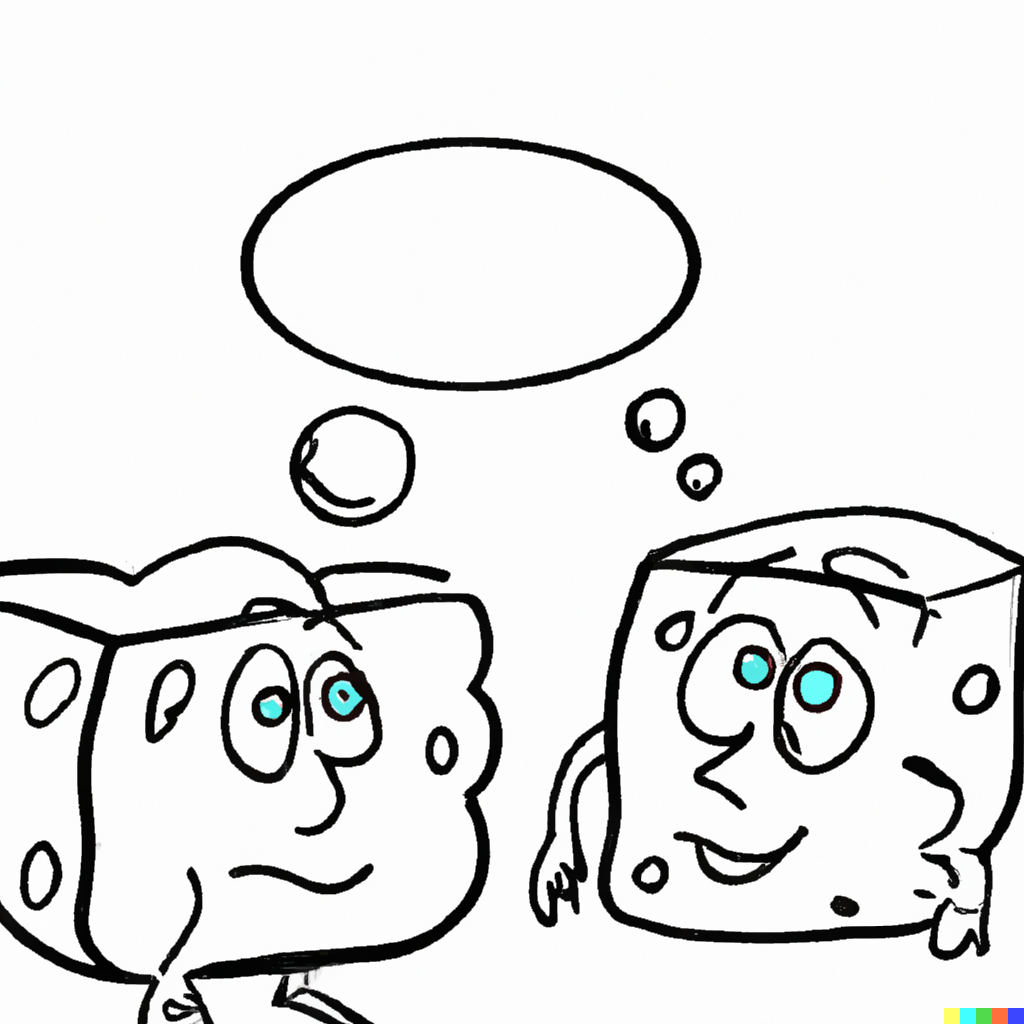
\includegraphics[width=5cm]{image/soaps-chatting}
    \end{frame}

    \begin{frame}
        \transdissolve
        \frametitle{SOA}
        \framesubtitle{Exercice \execcounterdispinc{}}
        \begin{tiny}
            Désigner et développer une architecture de services qui distribue les données de l'\href{https://www.data.gouv.fr/fr/datasets/index-egalite-professionnelle-f-h-des-entreprises-de-50-salaries-ou-plus/}{Index EgaPro}.
            Respecter les exigences suivantes~:
            \begin{itemize}
                \item Travailler par groupe de 3 maximum.
                \item Créer un repo GitHub dédié et le communiquer à l'enseignant.
                \item Chaque étudiant sera évalué selon ses commits sur le repo.
                Il doit développer au moins un service.
                \item Documenter l'architecture avec un diagramme de séquence.
                \item Documenter l'API REST avec un Swagger.
                \item Documenter l'API SOAP avec un WSDL~.
                \item Intégrer ces schémas à un README détaillé.
                \item Développer 3 services minimum~:
                \begin{itemize}
                    \begin{tiny}
                        \item Distribution des données EgaPro en RPC~.
                        \item Distribution des données EgaPro par API REST~.
                        \item Distribution des données EgaPro par API SOAP~.
                    \end{tiny}
                \end{itemize}
                \item Tous doivent avoir une base de donnée commune.
                \item Distribuer les données par SIREN suffit, voir \url{https://github.com/St-Michel-IT/testing/blob/master/egapro_api.py}.
                \item Configurer un Reverse Proxy (Nginx par exemple) pour avoir tous les services derrière le même domaine et port.
            \end{itemize}
            \begin{dangercolorbox}
                Le dernier commit de la journée sera évalué.
            \end{dangercolorbox}
        \end{tiny}
    \end{frame}
\end{document}
